\documentclass{article}

\usepackage{algorithm2e}
\usepackage{amsmath}
\usepackage{amssymb}
\usepackage{amsthm}
\usepackage{authblk}
\usepackage[english]{babel}
\usepackage{blkarray}
\usepackage[font=small]{caption}
\usepackage{cite}
\usepackage{enumerate}
\usepackage{graphicx}
\usepackage{url}

\setlength{\thickmuskip}{2mu plus 3mu minus 1mu}
\setlength{\medmuskip}{1mu plus 2mu minus 1mu}

\SetKwComment{Comment}{$\triangleright$\ }{}

% ---- Author affiliations ---- %

\renewcommand\Affilfont{\itshape\small}

% ---- Propositions, lemmas, defintions... ---- %

%\newtheorem{algorithm}{Algorithm}
\newtheorem{corollary}{Corollary}
\newtheorem{definition}{Definition}
%\newtheorem{example}{Example}
\newtheorem{lemma}{Lemma}
\newtheorem{proposition}{Proposition}
%\newtheorem{remark}{Remark}


% ---- Special environments (examples and remarks) ---- %

\newcounter{examplecounter}
\newenvironment{example}
{\small\vspace{0.5\baselineskip}
  \refstepcounter{examplecounter}%
  \noindent\textbf{Example \arabic{examplecounter}.}%
}{\vspace{-0.2\baselineskip}\begin{center}%
  $\star$\end{center}\vspace{0.5\baselineskip}}

\newcounter{remarkcounter}
\newenvironment{remark}
{\small\it\vspace{0.5\baselineskip}
  \refstepcounter{remarkcounter}%
  \noindent\textbf{Remark \arabic{remarkcounter}.}%
}{\vspace{0.5\baselineskip}}

\newenvironment{inset}
{\vspace{0.5\baselineskip}\begin{center}}
{\end{center}\vspace{0.5\baselineskip}}


% ---- Macros ---- %

\newcommand{\dn}[1]{\scriptstyle{\downarrow_{/#1}}}
\newcommand{\Dn}[1]{\scriptstyle{\Downarrow_{#1}}}
\newcommand{\up}[1]{\scriptstyle{\uparrow_{/#1}}}
\newcommand{\nd}{\scriptstyle{|}}
\newcommand{\modulo}[1]{\ (\mathrm{mod}\ #1)}

%---------------------------------------------------------------

\title{Calibrating seed-based alignment heuristics with Sesame}

\author[1,2]{Guillaume J. Filion}
\author[1]{Ruggero Cortini}
\author[1]{Eduard Zorita}
\affil[1]{Center for Genomic Regulation (CRG), The Barcelona Institute of
Science and Technology, Dr. Aiguader 88, Barcelona 08003, Spain.}
\affil[2]{University Pompeu Fabra (UPF), Barcelona, Spain.}

\date{\today}

%---------------------------------------------------------------
%---------------------------------------------------------------


\begin{document}

\maketitle

\begin{abstract}
% Statement of the problem.
The increasing throughput of DNA sequencing technologies creates a need
for faster algorithms. The fate of most reads is to be mapped to a
reference sequence, typically a genome. Modern mappers rely on heuristics
to gain speed at a reasonable cost for accuracy. In the seeding heuristic,
short matches between the reads and the genome are used to narrow the
search to a set of candidate locations. Several seeding variants used in
modern mappers show good empirical performance but they are difficult to
calibrate or to optimize for lack of theoretical results.
% Summary of the results.
Here we develop a theory to estimate the probability that the correct
location of a read is filtered out during seeding, resulting in mapping
errors. We describe the properties of simple exact seeds, skip-seeds and
MEM seeds (Maximal Exact Match seeds).
% Innovation.
The main innovation of this work is to use concepts from analytic
combinatorics to represent reads as abstract sequences, and to specify
their generative function to estimate the probabilities of interest.
% Durability.
We provide several algorithms, which combined together give a workable
solution for the problem of calibrating seeding heuristics for short
reads. We also provide a C implementation of these algorithms in a library
called Sesame.
% Scope.
These results can improve current mapping algorithms and lay the
foundation of a general strategy to tackle sequence alignment problems.
% Availability
The Sesame library is open source and available for download at
\url{https://github.com/gui11aume/sesame}.
\end{abstract}


%---------------------------------------------------------------
%---------------------------------------------------------------

\section{Introduction}

\subsection{Mapping reads to genomes}

Suppose that we use and imperfect instrument to sequence a DNA fragment
drawn at random from a known genome; how can we identify the location of
the fragment in the genome?

We will refer to this question as the \emph{true location problem}.
It has applications in countless domains, like discovering
disease-causing mutations; diagnosing viral, bacterial or fungal
infections; diagnosing cancer and choosing appropriate therapies;
selecting breeds of interest in agriculture; tracing human migrations from
ancient bones; diagnosing genetic diseases at birth; finding compatible
graft donors \textit{etc}.

At first sight, whether a read can be mapped to its correct location seems
to depend only on its length and on the error rate of the sequencer.
However, there is another important factor to consider: most genomes
contain repeated sequences, \textit{i.e.} relatively large subsequences
that are present at more than one location. For instance, we cannot map
the fragment with certainty if there exists an exact copy of the sequence
somewhere else in the genome, because we cannot know which of the two
copies was sequenced.

This case is rare though. Repeated sequences are in general not identical
but merely homologous --- meaning that their similarity is unlikely to
occur by chance. So when the DNA fragment has one or more duplicates in
the genome, we can still map it, as long as we can distinguish the
duplicates. This in turn depends on their similarity with the target
fragment and on the error rate of the sequencer.

Since repeats play a central role in the problem at hand, we give the
terms ``targets'' and ``duplicates'' a meaning that will facilitate the
exposition of the theory.

\begin{definition}
The target is the DNA fragment that was sequenced. Duplicates are
sequences of the genome that are homologous to the target.
\end{definition}

Because sequencing errors can convert the sequence of the target into one
of its duplicates, the \emph{true} location of a DNA fragment is not
always the \emph{best} candidate (as measured by the identity between the
sequence and the candidate location). This leads to the following
question: how can we identify the \emph{best} location of the fragment in
the genome? 

We will refer to this task as the \emph{best location problem}. It amounts
to finding the optimal alignment between two sequences, and for this
reason has received substantial attention in bioinformatics. For
simplicity we will assume that the true location is always the best, and
we will often confound these two ideas.

\subsection{Seeding heuristics}
\label{sec:seedheur}

There exist algorithms to solve the best location
problem~\cite{pmid7265238,pmid5420325}, but they are too slow to process
the large amount of data generated by modern sequencers. Instead, one uses
heuristic methods, \textit{i.e.} algorithms that run faster, but that may
return an incorrect result~\cite{Waterman1984}.

The most popular heuristic for the best location problem is a filtration
method called ``seeding''. The principle is to first identify short
regions of high similiarity between the read and the genome, and then run
an exact alignment algorithm at the candidate locations. This is for
instance the general strategy of the popular alignment algorithm
BLAST~\cite{pmid2231712}.

If seeding is fast, we can quickly zoom in on a small set of candidate
locations and reduce the input size of the (slow) alignment algorithm. The
disadvantage is that the target location is not always detected and
included in the candidate set. When that happens, the read cannot be
mapped to the true location because it has been filtered out at the
seeding step.

The slowness of exact alignment algorithms imposes a trade-off between
speed and accuracy: If the seeding step is set to produce many candidates,
it is likely to retrieve the true location. The downside is that
processing all the candidates would take long. Conversely, if the seeding
step is set to produce few candidates, the process would run faster but
the target is less likely to be in the candidate set.

Importantly, the trade-off depends on the seeding method. This means that
we can develop faster mapping algorithms at no cost for accuracy, as long
as we can find better seeding strategies. Progress on this line of
research has largely benefited from the improvement of computer hardware
and from the development of indexing algorithms. Literature on this topic
is already abundant. Some examples of seeding algorithms are given in
references~\cite{sun2005designing, pmid11934743, xu2006optimizing,
kucherov2005multiseed, brejova2003vector, pmid18684737, pmid15359419}.
References~\cite{pmid16533404} and~\cite{pmid20460430} present high-level
comparisons of different designs, and reference~\cite{navarro2001guided}
gives a global overview of filtration methods in pattern matching.

\subsection{The two types of seeding failure}
\label{sec:twotypes}

Filtering methods are considered to fail whenever the target is not in the
candidate set. For seeding heuristics, we need to distinguish two
different kinds of failure. In the first kind, the candidate set contains 
a duplicate of the target but does not contain the target itself; in the
second kind, the candidate set contains neither.

The distinction is important because duplicates of the target are similar
to the read (due to their similarity to the target), so a failure of the
first kind is difficult to distinguish from a success. A failure of the
second kind is easier to recognize because in this case the best hit is
not similar to the read, as we will highlight in
section~\ref{sec:random_seeds}.

Before going further, we introduce some nomenclature that will be useful
to simplify the exposition of the theory.

\begin{definition}
The seeding process is said to be
\begin{enumerate}[i)]
\item ``on target'' if the candidate set contains the target,
\item ``off target'' if the candidate set contains a duplicate but
not the target, 
\item ``null'' if the candidate set contains neither.
\end{enumerate}
\end{definition}

If a seed-based mapping algorithm returns an incorrect location, then it
must be the case that the best location was never tested in the
post-filtration phase (otherwise it would have been found by the exact
alignment algorithm).

This observation is fundamental: in order to estimate the error rate of a
mapping algorithm, we must know how often the associated seeding heuristic
is off target. For lack of theoretical framework, this information is
missing, meaning that current mappers are not properly calibrated.

Our focus here is to develop a theory to estimate the probability that
seeding is off target, when using the most popular seeding heuristics for
short reads. Previous work pioneered a method to compute seeding
probabilities but it did not distinguish off-target from null
seeding~\cite{filion2017analytic,filion2018analytic}, and therefore did
not provide a way to estimate the frequency of mapping errors. Other
authors investigated the reliability of mapping
algorithms~\cite{pmid23872968}, but they focused on the probability that
random sequences have a single hit, recognizing that solving the problem
requires taking into consideration the repeat structure of the genome.
Here we address this problem in general terms and we provide a practical
way to estimate the mismapping rate in complex genomes.

The rest of this document is not organized by logical units but by
increasing level of difficulty. The order of the examples is meant to
ease the acquisition of the main concepts, meaning that we sometimes go
back and forth between different types of seeding strategies. We first
give some background on the different types of seeding methods considered
here; we then introduce the computational strategy based on transfer
matrices; finally we delve into each specific seeding method.

\section{Seeds}

The term ``seed'' changes meaning with different authors. It can designate
a part of the read, a part of the genome, a particular sequence motif or a
structured pattern of matches. Also, the term does not always imply an
exact match. For instance, the algorithm PatternHunter~\cite{pmid11934743}
uses ``spaced seeds'' that tolerate mismatches. To avoid potential
confusion, we will adopt the following convention:

\begin{definition}
A seed is a subsequence of the read that has size at least $\gamma$
(defined by the context of the problem) and that has at least one perfect
match in the reference genome.
\end{definition}

When a seed matches a particular location of the genome, we say that it is
a ``seed for that location''. For instance, we often use expressions such
as ``a seed for the target'' or ``a seed for a duplicate''.

This definition presents a computational challenge: to know if a given
subsequence is a seed we need to know if it exists somewhere in the
genome. This is a non trivial problem in itself, but fortunately we can
use practical methods to solve it, even when the reference genome is very
large.

These algorithms are crucial for the present theory, but describing them
in depth is outside the scope of this document. Let us just mention that
all the methods belong to a family known as exact offline string matching
algorithms, where ``offline'' means that sequences are looked up in an
index instead of the genome itself. Online methods can be used when the
reference genome is not indexed~\cite{faro2013exact}, but this case is of
little relevance in the present context.

The index is usually a hash table or a variant of the so-called
FM-index~\cite{ferragina2000opportunistic, ferragina2005indexing}. Hash
tables are typically used to index $k$-mers, which makes them useful to
search seeds of fixed size $k$ (see~\cite{pmid30346548} for a recent
benchmark of $k$-mer hashing algorithms). In contrast, some text-indexing
structures have no set size so they can be used to search seeds of
different lengths. For instance, the FM-index is a compact data structure
based on the suffix array~\cite{manber1993suffix} and on the
Burrows-Wheeler transform~\cite{burrows1994block}, emulating a suffix trie
with a much smaller memory footprint~\cite{ferragina2000opportunistic,
ferragina2005indexing}.

Other methods can be efficient (\textit{e.g.}, running a bisection on the
suffix array~\cite{dobin2013star}) but the FM-index is currently the most
popular choice for seeding methods. For MEM seeds, it is even the only
practical option~\cite{pmid24336412, pmid25399029, pmid23349213,
pmid19389736}. However, the detail is of little interest here: we simply
assume that seeds are known at all times without ambiguity because this
problem has several practical solutions.


\subsection{Exact seeds}

Exact seeds have a fixed size $\gamma$. When using exact seeds, all the
perfect matches of size $\gamma$ are collected to constitute the candidate
set. This seeding heuristic was used in the first version of
BLASTN~\cite{pmid2231712}, but is no longer used because it produces many
overlapping matches within the same regions.

Fig.~\ref{fig:exact_seed_example} shows a read produced by an imperfect
sequencer. The sequenced DNA fragment comes from a region of the genome
that has three duplicates and the read has three miscalled nucleotides
(indicated by stars).

\begin{figure}[h]
\centering
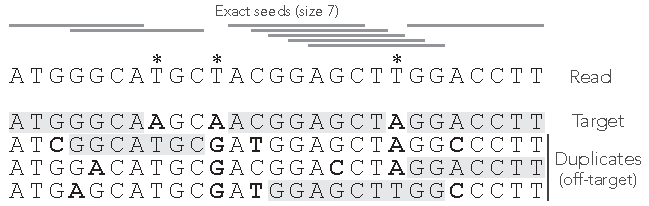
\includegraphics[scale=1]{exact_seed_example.pdf}
\caption{\textbf{Example of exact seeds.}
A sequenced DNA fragment (Read) is shown above the actual molecule
(Target), and above homologous sequences also present in the genome
(Duplicates). Sequencing errors are indicated by a star (each marked
\texttt{T} was actually an \texttt{A} that was misread). The mismatches
between the genomic sequences and the read are indicated in bold. The
exact seeds of size $\gamma = 7$ are indicated as horizontal grey lines
above the read. The matching regions in the genomic sequences are
shadowed in grey. Several overlapping seeds accumulate at the center of
the read, which is typical for this seeding method.}
\label{fig:exact_seed_example}
\end{figure}

Observe that erroneous nucleotides can belong to exact seeds because they
sometimes match one of the duplicates. For instance, the first sequencing
error matches all the duplicates and belongs to an off-target seed.
However, sequencing errors that are mismatches for \emph{all} the
sequences cannot belong to a seed. This is the case of the second
sequencing error in this example, where there is a local deficit of seeds.

The middle of the read shows some clutter where consecutive seeds
match consecutive sequences at the same location. This is typical for
exact seeds and constitutes a nuisance for the implementation. Indeed, it
is a waste of computer resources to discover matches in sequences that are
already in the candidate set. In addition, this seeding method is not
particularly sensitive compared to spaced seeds~\cite{pmid11934743} so it
is used only in few specific applications. Nevertheless, it will be
extremely useful for the development of the present theory.


\subsection{Skip seeds}

Skip seeds have a fixed size $\gamma$, but unlike exact seeds they cannot
start at every nucleotide. Instead, a certain amount of nucleotides is
skipped between every seed. This is a way to reduce the overlapping
matches at the same location, at the cost of sensitivity. This seeding
heuristic is the core of Bowtie2~\cite{pmid22388286}, where seeds have
size $\gamma=16$ and are separated by 10 nucleotides (9 positions are
skipped). We will refer to seeds where $n$ nucleotides are skipped as
``skip-$n$ seeds''. For instance, Bowtie2 uses skip-9 seeds.

\begin{figure}[h]
\centering
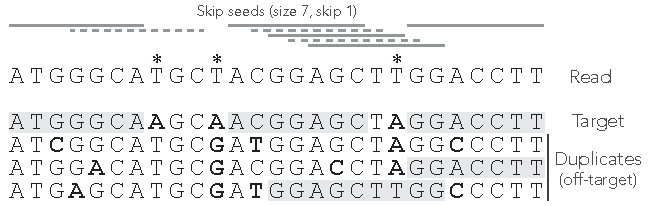
\includegraphics[scale=1]{skip_seed_example.pdf}
\caption{\textbf{Example of skip seeds.}
The sequences and the annotations are the same as in
Fig.~\ref{fig:exact_seed_example}, but here we use skip-1 seeds. In other
words, seeds can never start at nucleotides 2, 4, 6 \textit{etc}. To
highlight the difference with Fig.~\ref{fig:exact_seed_example}, the
missing seeds are represented by dotted lines.}
\label{fig:skip_seed_example}
\end{figure}

Fig.~\ref{fig:skip_seed_example} shows what happens when exact seeds are
replaced by skip-1 seeds on the read of Fig.~\ref{fig:exact_seed_example}.
Here the size is still $\gamma=7$ but 1 nucleotide is skipped between
seeds. This amounts to removing every second seed. The consequence is that
there are fewer overlapping matches at the center of the read, but the
only seed for the second duplicate is lost. This is a rather positive
outcome because there is one off-target location fewer in the candidate
set, but the same might happen to the target.

It is clear that skipping nucleotides reduces the sensitivity of the
seeding step, but to what extent? One could test this empirically, but the
answer depends on the seed length, the number of nucleotides that are
skipped, the error rate of the sequencer and the size of the reads. The
present theory will allow us to make general statements about the
performance of skip seeds against exact seeds in different contexts.


\subsection{MEM seeds}

MEM seeds (where MEM stands for Maximal Exact Match) are somewhat harder
to define. Unlike exact seeds and skip seeds, their size is variable. They
are used in BWA-MEM~\cite{li2013aligning} where they give good empirical
results. To describe MEM seeds, let us first clarify the meaning of
``Maximal Exact Match''.

\begin{definition}
A Maximal Exact Match (MEM) is a subsequence of the read that is present
in the reference genome and that cannot be extended --- either because the
read ends or because the extended subsequence is not in the genome.
\end{definition}

A \emph{MEM seed} is simply a MEM of size size $\gamma$ or greater.
Fig.~\ref{fig:MEM_example} shows what happens when using MEM seeds on the
read of Fig.~\ref{fig:exact_seed_example}. Observe that the clutter at the
center of the read has disappeared because consecutive matches are fused
into a few MEM seeds.

\begin{figure}[h]
\centering
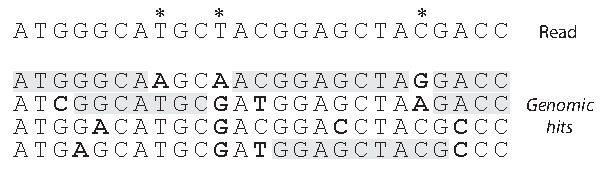
\includegraphics[scale=1]{MEM_example.pdf}
\caption{\textbf{Example of MEM seeds.}
The sequences and the annotations are the same as in
Fig.~\ref{fig:exact_seed_example}, but here we use MEM seeds of minimum
size $\gamma=7$. The clutter at the center of the read has disappeared and
there is at least one seed for each sequence.}
\label{fig:MEM_example}
\end{figure}

Two consecutive MEM seeds can overlap, in which case they always match
distinct sequences of the genome (otherwise neither of them would be a MEM
seed). There does not have to be any overlap though, because a nucleotide
can be a mismatch against \emph{all} the sequences, like the second read
error for instance.

Note that a MEM does not always match a single sequence of the genome. For
instance, the rightmost MEM seed matches two distinct genomic sequences.
This case motivates the following definition, which will play an important
role later.

\begin{definition}
A \emph{strict} MEM seed has a single match in the genome.
A \emph{shared} MEM seed has several matches in the genome.
\end{definition}

Compared to seeds of fixed size, MEM seeds have two counter-intuitive
properties. The first is that there are cases where there cannot be any
on-target seed, even when changing the sensitivity parameter $\gamma$.
Fig.~\ref{fig:full_masking_example} shows such an example. Even though
there is a single sequencing error, the read has no MEM seed for the
target. Lowering $\gamma$ does not change this, so there is no way to
discover the true location using MEM seeds (even though it is the best
location).

\begin{figure}[h]
\centering
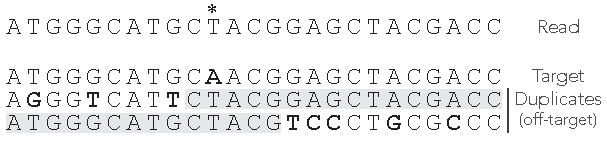
\includegraphics[scale=1]{full_masking_example.pdf}
\caption{\textbf{Issues with MEM seeds: inaccessible targets.}
The read, the MEM seeds and the sequences are represented as in
Fig.~\ref{fig:MEM_example}. The MEM seeds matching the two duplicates
at the bottom effectively hide the target, so it cannot be discovered.
This can occur even when the true location is the best candidate and when
there is a single error on the read.}
\label{fig:full_masking_example}
\end{figure}

The second counter-intuitive property is that shortening a read can
sometimes generate a MEM seed for the target. Fig.~\ref{fig:short_vs_long}
shows an example of this case. There is no MEM seed for the target, but
there would be if the read were two nucleotides shorter on the right
side. Indeed, in this case there would be a shared MEM seed matching the
the target and the first duplicate (provided $\gamma \leq 12$).


\begin{figure}[h]
\centering
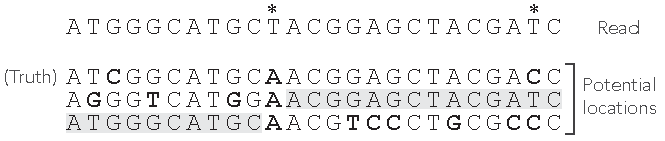
\includegraphics[scale=1]{short_vs_long_example.pdf}
\caption{\textbf{Issues with MEM seeds: too long reads.}
The read, the MEM seeds and the sequences are represented as in
Fig.~\ref{fig:MEM_example}. There would be a good seed (shared) if the
read were two nucleotides shorter. The true location is hidden by
the last two nucleotides.}
\label{fig:short_vs_long}
\end{figure}

These examples show that MEM seeds can perform worse than seeds of fixed
size. MEM seeds yield fewer candidates and therefore speed up the mapping
process, but the question is at what cost? The theory developed here will
allow us to compute the probability that a read has no MEM seed for the
target and thus that the true location is missed at the seeding stage.


\section{Model and strategy}
\label{sec:symbolic}

\subsection{Sequencing errors and divergence of the duplicates}
\label{sec:error}

We now need to model the sequencing and duplication processes so that
we can compute the probabilities of the events of interest. We assume that
the sequencing instrument has a constant substitution rate $p$, and that
insertions and deletions never occur. When a substitution occurs, we
assume that the instrument is equally likely to output any one of the
remaining three nucleotides. This corresponds more or less to the error
spectrum of the Illumina sequencing technology~\cite{pmid21576222}.

Next, we assume that the target sequence has $N \geq 0$ duplicates, so
that there are $N$ off-target sequences. We further assume that
duplication happened instantaneously at some point in the past and that
all $N+1$ sequences diverge independently of each other at a constant
rate. In other words, we ignore the complications due to the genealogy of
the duplication events. Instead, we simply assume that at each nucleotide
position, any given duplicate is identical to the target with probability
$1-\mu$. If it is not, we assume that the duplicate sequence can be any of
one the three remaining nucleotides (\textit{i.e.} each is found with
probability $\mu/3$).

Note that read errors are always mismatches against the target (because we
assume that the target is the true sequence), and they match each
duplicate with probability $\mu/3$. Correct nucleotides are always matches
for the target, and they match each duplicate with probability $1-\mu$.

Before going further, we also need to move a practical consideration out
of the way. Seeds can match any sequence of the genome, not just the
target or the duplicates. However, we will ignore matches in the rest of
the genome because such random matches are unlikely to cause a mapping
error when seeding is off target, contrary to matches in duplicates.
Neglecting those will greatly simplify the exposition of the theory
without loss of generality. We will explain in
section~\ref{sec:random_seeds} how to deal with this practical case and
and how to identify those matches as off target. Until then, we will
consider that the target and the duplicates are the only sequences in the
reference genome.


\subsection{Weighted generating functions}

The central object of analytic combinatorics is the generating function,
and for our purpose we will use a special kind known as \emph{weighted
generating function}.

\begin{definition}
\label{def:GF}
Let $\mathcal{A}$ be a set of combinatorial objects such that $a \in
\mathcal{A}$ has a size $|a| \in \mathbb{N}$ and a weight $w(a) \in
\mathbb{R}^+$. The weighted generating function of $\mathcal{A}$ is
defined as

\begin{equation}
\label{eq:GF1}
A(z) = \sum_{a \in \mathcal{A}} w(a) z^{|a|},
\end{equation}
Expression (\ref{eq:GF1}) also defines a sequence $(a_k)_{k \geq 0}$ such
that 

\begin{equation*}
A(z) = \sum_{k=0}^\infty a_k z^k.
\end{equation*}

By definition $a_k = \sum_{a \in A_k}w(a)$, where $A_k$ is the class of
objects of size $k$ in $\mathcal{A}$. The number $a_k$ is the
total weight of objects of size $k$.
\end{definition}

To give an example, assume that a particular symbol, say $\Downarrow$, has
a probability of occurence equal to $p$. The weighted generating function
words containing only this symbol is $pz$. The weight of the word is
its probability (here equal to $p$) and the size is its length in number
of symbols (here 1).

In this document we will focus on the weighted generating function $A(z)$
of the set $\mathcal{A}$ of reads that do not have on-target seeds
(\textit{i.e.} reads for which seeding is either null or off target). The
weight of a read is its probability of occurrence and the size $k$ is its
number of nucleotides. The coefficient $a_k$ is thus the proportion of
reads of size $k$ that do not have an on-target seed, which is the
quantity of interest.

The motivation for introducing weighted generating functions is that
operations on combinatorial objects translate into operations on their
weighted generating functions. If $A(z)$ and $B(z)$ are the weighted
generating functions of two mutually exclusive sets $\mathcal{A}$ and
$\mathcal{B}$, the weighted generating function of $\mathcal{A} \cup
\mathcal{B}$ is $A(z) + B(z)$, as evident from expression (\ref{eq:GF1}).
Size and weight can be defined for pairs of objects in $\mathcal{A} \times
\mathcal{B}$ as $|(a,b)| = |a| + |b|$ and $w(a,b) = w(a)w(b)$. In other
words the sizes are added and the weights are multiplied.  With this
convention, the weighted generating function of the Cartesian product
$\mathcal{A} \times \mathcal{B}$ is $A(z)B(z)$. This simply follows from
expression (\ref{eq:GF1}) and from

\begin{equation*}
A(z)B(z) =
\sum_{a\in \mathcal{A}}w(a)z^{|a|} \sum_{b\in \mathcal{B}}w(b)z^{|b|}
= \sum_{(a,b) \in \mathcal{A} \times \mathcal{B}} w(a)w(b)z^{|a|+|b|}.
\end{equation*}

These two operations are all we need in order to compute the weighted
generating functions of the reads of interest. Addition corresponds to
creating a new family by merging reads from families $\mathcal{A}$ and
$\mathcal{B}$. Multiplication corresponds to creating a new family by
concatenating reads from families $\mathcal{A}$ and $\mathcal{B}$.

\subsection{Analytic representation}

The analytic combinatorics framework relies on a strategy referred to as
the \emph{symbolic method}~\cite{sedgewick2013introduction}. The idea is
to combine simple objects into more complex objects. Each combinatorial
operation on the objects corresponds to a mathematical operation on their
weighted generating functions. One can thus obtain the weighted generating
function of complex objects, whose coefficients $a_k$ are the
probabilities of interest.

As explained in~\cite{filion2017analytic} and~\cite{filion2018analytic},
we recode the reads in alphabets of custom symbols and we specify a
construction plan of the reads using a \emph{transfer matrix} $M(z)$. The
transfer matrix specifies which types of segments can follow each other in
the reads of interest: the entry at coordinates $(i,j)$ is the weighted
generating function of segments of type $j$ that can be appended to
segments of type $i$.

$M(z)$ contains the weighted generating functions of all the reads that
consist of a single fragment. From the basic operations on weighted
generating functions, $M(z)^s$ contains the weighted generating functions
of all the reads that consist of $s$ segments. Therefore, the entry at
coordinates $(i,j)$ of the matrix $M(z) + M(z)^2 + M(z)^3 + \ldots = M(z)
\cdot (I-M(z))^{-1}$ is the weighted generating function of the reads of
any size and any number of segments, that end with a segment of type $j$
and that can be appended to a segment of type $i$. The examples below will
clarify the key steps of this strategy.

A complete description of how to compute seeding probabilities with the
symbolic method can be found in~\cite{filion2017analytic,
filion2018analytic}. The interested readers can also find more about
analytic combinatorics in the popular
textbooks~\cite{flajolet2009analytic, sedgewick2013introduction}.


\subsection{Example 1: on-target exact seeds}
\label{sec:example_exact}

We highlight the strategy above with an example that will turn out to be
central for the development of the theory. In addition, it is simple
enough to provide a gentle introduction to the general methodology. This
example was described in detail in~\cite{filion2017analytic} and
in~\cite{filion2018analytic}, but we repeat it here with a different
formalism to fit the present manuscript.

The first step is to note that the nucleotide sequence of the read is
irrelevant. Indeed, the read has an on-target seed if and only if it
contains a stretch of $\gamma$ nucleotides without error. For this reason,
we recode reads as sequences of correct or erroneous nucleotides.

We define the mismatch alphabet $\mathcal{A}_0 = \{\square, |,
\Downarrow\}$, where $\square$ represents a correct nucleotide,
$\Downarrow$ represents an erroneous nucleotide and $|$ is special symbol
appended after the last nucleotide to mark the end of the read. It is not
associated to a nucleotide and therefore has size 0.

This recoding allows us to partition the read in an important way.

\begin{definition}
\label{def:seg}
Every symbol of the alphabet that is different from $\square$ is called a
terminator. A segment is a terminator preceded by 0 or more symbols $\square$.
The last segment of the read is terminated by the symbol $|$ and is called the
tail.
\end{definition}

Since the decomposition of the read in segments is unique, we can view a
read as a sequence of segments with a tail, instead of a sequence of
nucleotides. Fig.~\ref{fig:simple} shows an example of decomposition in
segments. On-target seeds cannot contain sequencing errors, therefore they
must be completely embedded inside a segment. So the sizes of the segments
indicate whether the read contains an on-target seed or not.

\begin{figure}[h]
\centering
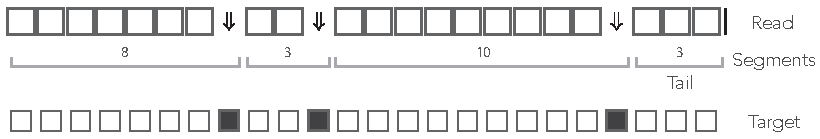
\includegraphics[scale=0.85]{sketch_simple.pdf}
\caption{\textbf{The mismatch encoding.}
An example read is represented in the mismatch alphabet. The symbol
$\Downarrow$ represents a mismatch against the target (an erroneous
nucleotide) and the symbol $\square$ represents a match (a correct
nucleotide). The symbol $|$ is appended to the end of the read. The
symbolic sequence of the target is represented below, where an open square
stands for a match and a closed square stands for a mismatch.}
\label{fig:simple}
\end{figure}

The probability of occurrence of the symbol $\Downarrow$ is $p$ (the error
rate of the sequencer) and the probability of occurrence of the symbol
$\square$ is thus $1-p = q$. Both symbols have size 1, so their respective
weighted generating function are $pz$ and $qz$. Using the rule for
concatenation, we see that the weighted generating function of a segment
with $i$ symbols $\square$ is $(qz)^ipz$. The symbol $|$ has size 0, so
the weighted generating function of a tail segment with $i$ symbols
$\square$ is $(qz)^i$.

The key insight is that reads without on-target seed are exactly the reads
that are made of segments with fewer than $\gamma$ symbols $\square$. The
weighted generating function of such segments is $pz \cdot \big(
1+qz+\ldots+(qz)^{\gamma-1} \big)$, and that of the tail is
$1+qz+\ldots+(qz)^{\gamma-1}$. This gives a construction plan that can be
encoded in a transfer matrix.

There are two kinds of objects: the $\Downarrow$ segments and the tails,
so the dimension of the transfer matrix is $2 \times 2$. A $\Downarrow$
segment can be followed by another $\Downarrow$ segment or by the tail.
The tail cannot be followed by anything. The expression of the transfer
matrix $M_0(z)$ is thus
\begin{equation*}
\begin{blockarray}{ccc}
   & \scriptstyle{\Downarrow} & \scriptstyle{|} \\
\begin{block}{c[cc]}
\scriptstyle{\Downarrow} & pz \cdot \big( 1+qz+\ldots+(qz)^{\gamma-1}
\big)  & 1+qz+\ldots+(qz)^{\gamma-1} \\
\scriptstyle{|} & 0 & 0 \\
\end{block}
\end{blockarray}.
\end{equation*}

In the representation above, the different types of objects are identified
by their terminator. The terminators are written in the margins of the
transfer matrix for readability.

We can compute the matrix $M_0(z) + M_0(z)^2 + \ldots = M_0(z) \cdot
(I-M_0(z))^{-1}$ and extract the entry of interest, which is the top right
term --- associated with terminators $\Downarrow$ and $|$. To see why,
observe that every read can be prepended by $\Downarrow$ segments and only
by those (not by a tail). Thus, reads are precisely the sequences of
segments that can follow the symbol $\Downarrow$ and that are terminated
by a tail, whose weighted generating function is the top right entry of
the matrix. It is easy to check that this term is equal to
\begin{equation}
\label{eq:F}
\frac{1+qz+\ldots+(qz)^{\gamma-1}}
  {1-pz \big(1+qz+\ldots+(qz)^{\gamma-1} \big)}.
\end{equation}

This function can be expanded as a Taylor series $a_0 + a_1z + a_2z^2 +
\ldots$, but the coefficients $a_0, a_1, a_2, \ldots$ are unknown. By
construction, $a_k$ is the quantity of interest, \textit{i.e.} it is the
probability that a read of size $k$ does not contain an on-target seed, so
we now need to extract the coefficients from expression (\ref{eq:F}).
There are several methods to do so; the one we choose here is to build a
recurrence equation to compute $a_k$ from the previous terms of the series
$a_0, a_1, \ldots, a_{k-1}$. For this, we observe that for $z \neq 1/q$,
equation
\begin{equation*}
\frac{1+qz+\ldots+(qz)^{\gamma-1}}
  {1-pz \big(1+qz+\ldots+(qz)^{\gamma-1} \big)} =
  a_0 + a_1z +a_2z^2 + \ldots
\end{equation*}
is equivalent to
\begin{equation*}
(1-qz) \left(1-pz \big(1+qz+\ldots+(qz)^{\gamma-1} \big)\right)
(a_0 + a_1z +a_2z^2 + \ldots) = 1-(qz)^\gamma.
\end{equation*}
Balancing the terms of same degree on both sides of the equation leads
to the following relationship between the coefficients of the series:
\begin{equation}
\label{eq:recur}
a_k = 
\begin{cases}
1            &\quad\text{if } k < \gamma, \\
1 -q^\gamma &\quad\text{if } k = \gamma, \\
a_{k-1} -pq^\gamma \cdot a_{k-\gamma-1} &\quad\text{otherwise.}
\end{cases}
\end{equation}

These results are consistent: for $k < \gamma$, the read is too short so
the probability that it contains no seed is 1; for $k = \gamma$, the
read contains a seed if and only if it has no error, which occurs with
probability $q^\gamma$.

The terms of interest can be computed recursively using expression
(\ref{eq:recur}). This approach is very efficient because every iteration
involves at most one multiplication and one subtraction. Also, the default
floating-point arithmetic on modern computers gives sufficient precision
to not worry about numeric instability for the problems considered here
(we rarely need to compute those probabilities for reads above 500
nucleotides).

This example shows how the symbolic approach yields a non-trivial and yet
simple algorithm to compute the probability that a read of size $k$ does
not contain an on-target exact seed.


\subsection{Example 2: on-target skip seeds}
\label{sec:example_skip}

We go through another essential example, namely we devise a method to
compute the probability that a read contains no on-target skip seed. Using
the same strategy as in the previous example, we start by recoding the
reads using a specialized alphabet to solve this problem.

As in the previous example, we need to know whether a nucleotide is a
sequencing error, but this time we also need to know its phase in the
repeated cycles of skipped positions. For this, we define the skip-$n$
alphabet $\mathcal{A}_n = \{\square, |, \Downarrow_0, \Downarrow_1,
\ldots, \Downarrow_n \}$. Again, the symbol $\square$ represents a correct
nucleotide and the symbol $|$ is a terminator added at the end of the
read. The symbols $\Downarrow_i$ ($i \in \mathbb{N}$) represent sequencing
errors and $i$ indicates the number of nucleotides till the next
non-skipped position (\textit{i.e.} $i=0$ for nucleotides immediately
before a non-skipped position and $i=n$ for nucleotides at a non-skipped
position).

As per definition~\ref{def:seg}, segments in this alphabet are sequences
of 0 or more symbols $\square$ followed by any of the symbols
$\Downarrow_i$ or by the symbol $|$. Given that this decomposition is
unique, we can again view a read as a sequence of segments with a tail.
The example of Fig.~\ref{fig:simple} is shown again in
Fig.~\ref{fig:skip}, where segments in the mismatch alphabet have been
replaced by segments in the skip-3 alphabet.

\begin{figure}[h]
\centering
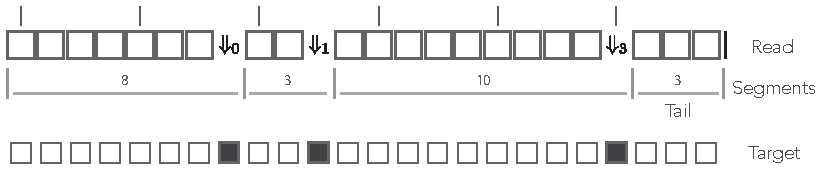
\includegraphics[scale=0.85]{sketch_skip.pdf}
\caption{\textbf{The skip encoding.}
The read of Fig.~\ref{fig:simple} is represented in the skip-3 alphabet.
The symbols $\Downarrow_i (i = 1,2,3)$ represent mismatches against the
target (they are erroneous nucleotides) and the symbol $\square$
represents a match (it is a correct nucleotide). The vertical bars
indicate non-skipped positions (the potential start of a seed). The number
$i$ in $\Downarrow_i$ indicates the number of nucleotides till the next
non-skipped position. For $i=0$ the next nucleotide is not skipped.
Other features are as in Fig.~\ref{fig:simple}.}
\label{fig:skip}
\end{figure}

The probability of occurrence of a sequencing error is $p$, so every
symbol $\Downarrow_i$ has the same weighted generating function $pz$ ---
implicitly assuming that the next non-skipped position is at distance $i$,
otherwise the weighted generating function is 0. The weighted generating
function of the symbol $\square$ is again $qz$, and so the weighted
generating function of a segment with $i$ symbols $\square$ is $(qz)^ipz$.
Likewise, the weighted generating function of a tail with $i$ symbols
$\square$ is $(qz)^i$.

Reads that do not contain any on-target skip seed can contain segments
with $\gamma$ or more symbols $\square$, so this case is more complex than
the previous one. For instance, if there is a sequencing error $i$
nucleotides before the next non-skipped position, the status of the next
$i$ nucleotides does not have any influence on the presence of an
on-target seed. Indeed, there is no on-target seed upstream of the error
(by construction) and the next seed is scheduled to start $i$ nucleotides
downstream, so there can be up to $\gamma+i-1$ symbols $\square$ in a row.
In order to enforce the absence of on-target seeds, we thus have to adjust
the maximum size of the segments depending on the preceding terminator.

In the skip-$n$ alphabet, reads are composed of segments terminated by the
$n+1$ symbols $\Downarrow_0, \Downarrow_1, \ldots, \Downarrow_n$, plus the
tail. The dimensions of the transfer matrix are thus $(n+2) \times (n+2)$.

As mentioned above, after the terminator $\Downarrow_i$, we can append
segments with up to $\gamma+i-1$ symbols $\square$. The terminators of
those $\gamma+i$ possible segments are distributed according to the laws
of the arithmetic modulo $n+1$. When $i > 0$, for instance, if the next
segment has no symbol $\square$ then it is terminated by
$\Downarrow_{i-1}$. But the same goes if the segment has $n+1$ symbols
$\square$ (assuming $n+1 < \gamma$). Specifying the transfer matrix thus
involves a substantial amount of bookkeeping. One can check that the
expression of the transfer matrix $M_n(z)$ is
\begin{equation*}
\begin{blockarray}{cccccc}
   & \Dn{0} & \Dn{1} & \ldots & \Dn{n} & \nd \\
\begin{block}{c[ccccc]}
\Dn{0} & H_{0,0}(z) & H_{0,1}(z) & \ldots & H_{0,n}(z) & J_0(z) \\
\Dn{1} & H_{1,0}(z) & H_{1,1}(z) & \ldots & H_{1,n}(z) & J_1(z) \\
\vdots & \vdots & \vdots & \ddots & \vdots & \vdots \\
\Dn{n} & H_{n,0}(z) & H_{n,1}(z) & \ldots & H_{n,n}(z) & J_n(z) \\
\nd & 0 & 0 & \ldots & 0 & 0 \\
\end{block}
\end{blockarray},
\end{equation*}
\begin{eqnarray}
H_{i,j}(z) &=& pz \cdot (qz)^x \cdot \big( 1 + (qz)^{n+1} +
  \ldots + (qz)^{m(n+1)} \big), \\
\notag
  &\;& \text{where } x = i-j-1 \modulo{n+1},
  \text{ and } m = \left\lfloor
  \frac{\gamma+i-1-x}{n+1} \right\rfloor, \\
J_i(z) &=& 1 + qz + (qz)^2 + \ldots + (qz)^{\gamma+i-1},
\end{eqnarray}
where $\lfloor \ldots \rfloor$ denotes the ``floor'' function.

The weighted generating function of interest is the top right entry of the
matrix $M_n(z) + M_n(z)^2 + \ldots = M_n(z)\cdot(I-M_n(z))^{-1}$. To see
why, observe that, at the start of every read, the next nucleotide is a
non-skipped position, so every read can be prepended by $\Downarrow_0$
segments and only by those. Thus, reads are precisely the sequences of
segments that can follow the symbol $\Downarrow_0$ and that are terminated
by a tail, whose weighted generating function is the entry of the matrix
associated with terminators $\Downarrow_0$ and $|$.

$M_n(z)$ is too complex to allow a closed expression of $M_n(z) \cdot
(I-M_n(z))^{-1}$ to be computed. We return to the definition $M_n(z) +
M_n(z)^2 + \ldots$ and observe that the terms $M_n(z)^{k+2}, M_n(z)^{k+3},
\ldots$ have no influence on the coefficients of the weighted generating
function $a_0, a_1, \ldots, a_k$.

Indeed, a read of size $k$ has at most $k+1$ segments (including the
obligatory tail). Since $M(z)^{s+1}$ contains the weighted generating
functions of reads with exactly $s+1$ segments including the tail, $a_k$
cannot depend on $M(z)^{k+2}, M(z)^{k+3}, \ldots$. More formally, we can
prove by induction that all the entries of $M(z)^k$ are divisible by
$z^{k-1}$, showing that the contribution of $M(z)^{k+2} + M(z)^{k+3} +
\ldots$ to $a_0 + a_1z + \ldots +a_kz^k$ is strictly $0$.

So we can compute the matrix $M_n(z) + M_n(z)^2 + \ldots + M_n(z)^{k+1}$,
extract the entry of interest and then compute the terms of the Taylor
expansion up to order $k$. But we can do better: since we are only
interested in the coefficients up to order $k$, we can perform all
algebraic operations on truncated polynomials of order $k$, \textit{i.e.}
we discard the coefficients of order $k+1$ or greater when multiplying two
polynomials.

But we can do even better: a read with $s+1$ segments contains $s$ errors,
so all the entries of $M_n(z)^{s+1}$ are dominated by $p^s$ and they
rapidly converge to $0$ as $s$ increases. Instead of computing the matrix
$M_n(z) + M_n(z)^2 + \ldots + M_n(z)^{k+1}$, we can interrupt the
summation after a certain power of $M_n(z)$ because the terms become
negligible.

The number of errors $X$ in a read of size $k$ has a Binomial
distribution $X \sim B(k,p)$. From~\cite{arratia1989tutorial} we can bound
the probabilities of the tail with the expression

\begin{equation}
\label{eq:bound}
Pr(X \geq s) \leq \exp \left( (s-k)\log \frac{k-s}{k(1-p)} -s\log
\frac{s}{kp} \right).
\end{equation}

Using the formula above, we can thus bound the probability that a read has
$s+1$ segments or more. We compute $M_n(z) + M_n(z)^2 + \ldots
+M_n(z)^{s+1}$ where the weighted generating functions have been replaced
by truncated polynomials and we extract the top right entry. When the
bound is lower than a set fraction $\varepsilon$ of the current value of
$a_k$, we stop the computations. Typically $\varepsilon = 0.01$ so this
method ensures that the probabilities that a read of size $k$ has no
on-target skip seed are accurate to within 1\%.

\begin{remark}
Observe that when $n=0$ the matrix $M_n(z)$ is identical to the matrix
$M_0(z)$ of section~\ref{sec:example_exact}. This is consistent with the
fact that exact seeds are skip-$0$ seeds.
\end{remark}

\section{Off-target exact seeds}
\label{sec:offexact}

We now turn our attention to the problem of computing the probability that
the seeding process is off target when using exact seeds --- recall from
section~\ref{sec:twotypes} that off-target seeding means that the
candidate set contains a duplicate but not the target.

If there is $N = 0$ duplicate, seeding cannot be off target, it can only
be on target or null. So from here we assume that the target has $N \geq
1$ duplicates. Let $S_0$ denote the event that there is an on-target seed
and let $S_j$ denote the event that there is a seed for the $j$-th
duplicate. We are thus interested in computing $P\big(\overline{S}_0 \cap
(S_1 \cup \ldots \cup S_N)\big)$, where $\overline{S}_j$ denotes the
complement of the event $S_j$. For this, we first observe that
\begin{equation}
\label{eq:pcomp}
P\big(\overline{S}_0 \cap (S_1 \cup \ldots \cup S_N)\big) =
P(\overline{S}_0) - P\big(\overline{S}_0 \cap \overline{S}_1 \cap \ldots
\cap \overline{S}_N\big).
\end{equation}

Since the duplicates are assumed to evolve independently of each other and
through the same mutagenesis process, the events are conditionally
independent (we do not have full independence because $S_0$ only depends
on sequencing errors whereas the events $S_j$ depend on sequencing errors
and on the divergence between duplicates). We can thus write
\begin{eqnarray}
\notag
P(\overline{S}_0 \cap \ldots \cap \overline{S}_N) &=&
  P(\overline{S}_0) \cdot P(\overline{S}_1 \cap \ldots \cap
  \overline{S}_N | \overline{S}_0) \\
\label{eq:Pnull}
  &=& P(\overline{S}_0) \cdot P(\overline{S}_1 | \overline{S}_0)^N =
  P(\overline{S}_0) \cdot \left( \frac{P(\overline{S}_0 \cap
\overline{S}_1)}{P(\overline{S}_0)} \right)^N.
\end{eqnarray}
Combinging the two equations above, we obtain
\begin{equation}
\label{eq:Poff}
P\big(\overline{S}_0 \cap (S_1 \cup \ldots \cup S_N)\big) =
P(\overline{S}_0) - P(\overline{S}_0) \cdot \left( \frac{P(\overline{S}_0
\cap \overline{S}_1)}{P(\overline{S}_0)} \right)^N.
\end{equation}

Hence, the probability that seeding is off target is a function of two
quantitites. We have already seen how to compute $P(\overline{S}_0)$ in
section~\ref{sec:example_exact} using recursive expression
(\ref{eq:recur}). We now need to find a way to compute $P(\overline{S}_0
\cap \overline{S}_1)$.

\subsection{The dual encoding}
\label{sec:dual}

The event $\overline{S}_0 \cap \overline{S}_1$ is that the read contains
no seed for either the target or for the first duplicate --- numbering is
arbitrary here, we simply chose a duplicate and stick to it. As
illustrated in section~\ref{sec:symbolic}, we first recode the reads using
a specialized alphabet to simplify the problem.

It will be useful to consider a more general problem where we
have two sequences of interest labelled $+$ and $-$. The $+$ sequence
stands for the target and that the $-$ sequence stands for its duplicate.
We then define the dual alphabet $\tilde{\mathcal{A}}_0 = \{\square, |,
\downarrow_{/1}^-, \downarrow_{/2}^-, \ldots, \downarrow_{/1}^+,
\downarrow_{/2}^+, \ldots, \Downarrow\}$. The symbols $\downarrow_{/i}^-$
signify that the nucleotide is a mismatch against the $-$ sequence only,
the symbols $\downarrow_{/i}^+$ signify that it is a mismatch against the
$+$ only, and the symbol $\Downarrow$ signifies that it is a mismatch
against both. As before, every other nucleotide is replaced by the symbol
$\square$, and the terminator $|$ is appended to the end of the read. We
again define reads as sequences of segments, except that now the
terminators are the symbols $\downarrow_{/j}^-$, $\downarrow_{/j}^+$ and
$\Downarrow$. The tail, as usual, is terminated by the symbol $|$.

The number $i$ in the symbol $\downarrow_{/i}^-$ indicates the match
length of the $+$ sequence. Likewise, the number $i$ in the symbol
$\downarrow_{/i}^+$ indicates the match length of the $-$ sequence. For
instance, the symbol $\downarrow_{/7}^-$ indicates that the nucleotide is a
mismatch against the $-$ sequence, that it is a match for the $+$
sequence, and that the six previous nucleotides were also a match for the
$+$ sequence. The terminators thus encode the local state of the read.

Fig.~\ref{fig:dual} shows an example of read in the dual encoding. The $+$
and $-$ sequences are represented below the read, with matches represented
as open squares and mismatches as closed squares. It is visible from this
example that symbols $\downarrow^-_{/i}$ and $\downarrow^+_{/i}$ alternate
whenever the mismatches hit different sequences . The symbol $\Downarrow$
occurs only when a nucleotide is a double mismatch.

\begin{figure}[h]
\centering
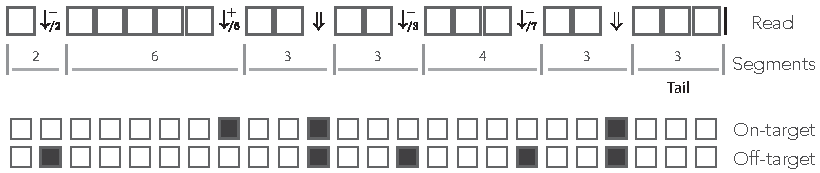
\includegraphics[scale=0.85]{sketch_dual.pdf}
\caption{\textbf{Example of dual encoding.}
An example of read is represented in the dual alphabet. The symbols
$\downarrow_{/i}^-$ represent a mismatch against the $-$ sequence, the
symbols $\downarrow_{/i}^+$ represent a mismatch against the $+$ sequence,
and the symbol $\Downarrow$ represent a mismatch against both. The index
$i$ is the match length of the sequence that is not mismatched. The
symbolic $+$ and $-$ sequences are represented below, where an open square
stands for a match and a closed square stands for a mismatch.}
\label{fig:dual}
\end{figure}

We assume that for each nucleotide, $a$ is the probability that the read
matches both sequences, $b$ is the probability that it matches only the
$+$ sequence, $c$ is the probability that it matches only the $-$ sequence
and $d$ is the probability that it matches none. Obviously $a+b+c+d=1$.
These definitions allow us to specify the weighted generating function of
the symbols and of the segments. To specify the transfer matrix, we only
have to make sure that we eliminate the combinations that create a match
of size $\gamma$ or more for any of the two sequences. For notational
convenience, we define
\begin{equation*}
\begin{gathered}
r_i^+(z) = cz \cdot (az)^i, \\
r_i^-(z) = bz \cdot (az)^i, \\
R_i(z) = dz \cdot \big( 1 + az + \ldots + (az)^i \big), \\
F_i(z) = 1 + az + \ldots + (az)^i,
\end{gathered}
\end{equation*}
and we can verify that the expression of the transfer matrix
$\tilde{M}_0(z)$ is
\begin{equation*}
\begin{blockarray}{ccccccccc}
   & \scriptstyle{\Downarrow} & \scriptstyle{\downarrow_{/1}^+} & 
    \ldots & \scriptstyle{\downarrow_{\gamma-1}^+} &
    \scriptstyle{\downarrow_{/1}^-} & \ldots &
    \scriptstyle{\downarrow_{/\gamma-1}^-} & \scriptstyle{|} \\
\begin{block}{c[cccccccc]}
\scriptstyle{\Downarrow} & R_{\gamma-1}(z)  & r_0^+(z) & \ldots &
    r_{\gamma-2}^+(z) & r_0^-(z) & \ldots & r_{\gamma-2}^-(z) &
    F_{\gamma-1}(z) \\
\scriptstyle{\downarrow_{/1}^+} & R_{\gamma-2}(z) & & & & & & &
    F_{\gamma-2}(z) \\
\scriptstyle{\downarrow_{/2}^+} & R_{\gamma-3}(z) & & & & & & &
    F_{\gamma-3}(z) \\
\vdots & \vdots & & \tilde{A}(z) & & & \tilde{B}_0(z) & & \vdots \\
\scriptstyle{\downarrow_{/\gamma-1}^+} & R_0(z) & & & & & & & F_0(z) \\
\scriptstyle{\downarrow_{/1}^-} & R_{\gamma-2}(z) & & & & & & &
    F_{\gamma-1}(z) \\
\scriptstyle{\downarrow_{/2}^+} & R_{\gamma-3}(z) & & & & & & &
    F_{\gamma-2}(z) \\
\vdots & \vdots & & \tilde{C}_0(z) & & & \tilde{D}(z) & & \vdots \\
\scriptstyle{\downarrow_{/\gamma-1}^+} & R_0(z) & & & & & & & F_0(z) \\
\scriptstyle{|} & 0 & 0 & \ldots & 0 & 0 & \ldots & 0 & 0 \\
\end{block}
\end{blockarray},
\end{equation*}
where $\tilde{A}(z)$, $\tilde{B}_0(z)$, $\tilde{C}_0(z)$ and
$\tilde{D}(z)$ are matrices of dimensions $(\gamma-1) \times (\gamma-1)$
that are defined as
\begin{equation*}
\tilde{A}(z) = 
\begin{blockarray}{cccccc}
   & \scriptstyle{\downarrow_{/1}^+} & \scriptstyle{\downarrow_{/2}^+} &
    \ldots & \scriptstyle{\downarrow_{/\gamma-2}^+} &
    \scriptstyle{\downarrow_{/\gamma-1}^+} \\
\begin{block}{c[ccccc]}
\scriptstyle{\downarrow_{/1}^+} & 0 & r_0^+(z) & \ldots &
    r_{\gamma-4}^+(z) & r_{\gamma-3}^+(z) \\
\scriptstyle{\downarrow_{/2}^+} & 0 & 0 & \ldots &
    r_{\gamma-5}^+(z) & r_{\gamma-4}^+(z) \\
\vdots & \vdots & \vdots & \ddots & \vdots & \vdots \\
\scriptstyle{\downarrow_{/\gamma-2}^+} & 0 & 0 & \ldots & 0 & r_0^+(z) \\
\scriptstyle{\downarrow_{/\gamma-1}^+} & 0 & 0 & \ldots & 0 & 0 \\
\end{block}
\end{blockarray},
\end{equation*}
\begin{equation*}
\tilde{B}_0(z) = 
\begin{blockarray}{cccccc}
   & \scriptstyle{\downarrow_{/1}^-} & \scriptstyle{\downarrow_{/2}^-} &
   \ldots & \scriptstyle{\downarrow_{/\gamma-2}^-} &
   \scriptstyle{\downarrow_{/\gamma-1}^-} \\
\begin{block}{c[ccccc]}
\scriptstyle{\downarrow_{/1}^+} & r_0^-(z) & r_1^-(z) & \ldots &
    r_{\gamma-3}^-(z) & r_{\gamma-2}^-(z) \\
\scriptstyle{\downarrow_{/2}^+} & r_0^-(z) & r_1^-(z) & \ldots &
    r_{\gamma-3}^-(z) & 0 \\
\vdots & \vdots & \vdots & \ddots & \vdots & \vdots \\
\scriptstyle{\downarrow_{/\gamma-2}^+} & r_0^-(z) & r_1^-(z) &
    \ldots & 0 & 0 \\
\scriptstyle{\downarrow_{/\gamma-1}^+} & r_0^-(z) & 0 & \ldots & 0 & 0 \\
\end{block}
\end{blockarray},
\end{equation*}
\begin{equation*}
\tilde{C}_0(z) = 
\begin{blockarray}{cccccc}
   & \scriptstyle{\downarrow_{/1}^+} & \scriptstyle{\downarrow_{/2}^+} &
    \ldots & \scriptstyle{\downarrow_{/\gamma-2}^+} &
    \scriptstyle{\downarrow_{/\gamma-1}^+} \\
\begin{block}{c[ccccc]}
\scriptstyle{\downarrow_{/1}^-} & r_0^+(z) & r_1^+(z) & \ldots &
    r_{\gamma-3}^+(z) & r_{\gamma-2}^+(z) \\
\scriptstyle{\downarrow_{/2}^-} & r_0^+(z) & r_1^+(z) & \ldots &
    r_{\gamma-3}^+(z) & 0 \\
\vdots & \vdots & \vdots & \ddots & \vdots & \vdots \\
\scriptstyle{\downarrow_{/\gamma-2}^-} & r_0^+(z) & r_1^+(z) & \ldots &
    0 & 0 \\
\scriptstyle{\downarrow_{/\gamma-1}^-} & r_0^+(z) & 0 & \ldots & 0 & 0 \\
\end{block}
\end{blockarray},
\end{equation*}
\begin{equation*}
\tilde{D}(z) = 
\begin{blockarray}{cccccc}
   & \scriptstyle{\downarrow_{/1}^-} & \scriptstyle{\downarrow_{/2}^-} &
    \ldots & \scriptstyle{\downarrow_{/\gamma-2}^-} &
    \scriptstyle{\downarrow_{/\gamma-1}^-} \\
\begin{block}{c[ccccc]}
\scriptstyle{\downarrow_{/1}^-} & 0 & r_0^-(z) & \ldots &
    r_{\gamma-4}^-(z) & r_{\gamma-3}^-(z) \\
\scriptstyle{\downarrow_{/2}^-} & 0 & 0 & \ldots &
    r_{\gamma-5}^-(z) & r_{\gamma-4}^-(z) \\
\vdots & \vdots & \vdots & \ddots & \vdots & \vdots \\
\scriptstyle{\downarrow_{/\gamma-2}^-} & 0 & 0 & \ldots & 0 & r_0^-(z) \\
\scriptstyle{\downarrow_{/\gamma-1}^-} & 0 & 0 & \ldots & 0 & 0 \\
\end{block}
\end{blockarray}.
\end{equation*}

The term of interest is the top right entry of
$\tilde{M}_0(z)\cdot(I-\tilde{M}_0(z))^{-1}$. To see why, observe that
every read can be prepended by $\Downarrow$ segments and only by those
(every other terminator would imply that one of the two sequences has a
nonzero match size at the start of the read). Thus reads are precisely the
sequences of segments that can follow the symbol $\Downarrow$ and that are
terminated by a tail, whose weighted generating function is the top right
entry of the matrix.

$\tilde{M}_0(z)$ is too complex to allow a closed expression of
$\tilde{M}_0(z)\cdot(I-\tilde{M}_0(z))^{-1}$ to be computed. It is
actually easier to proceed as in section~\ref{sec:example_skip} and to
compute the powers of $\tilde{M}_0(z)$ (using the arithmetic of truncated
polynomials) up to a given threshold value. Since each segment except the
tail contains a mismatch against at least one sequence, we define
$\tilde{p}$ as the upper bound on the probability of a mismatch $\tilde{p}
= \max\{b,c,d\}$. The updated formula (\ref{eq:bound}) now gives an upper
bound of the probability that a read of size $k$ contains $s$ or more
mismatches as
\begin{equation*}
Pr(X \geq s) \leq \exp \left( (s-k)\log \frac{k-s}{k(1-\tilde{p})} -s\log
\frac{s}{k\tilde{p}} \right).
\end{equation*}

Now returning to the problem of computing $P(\overline{S}_0 \cap
\overline{S}_1)$, the $+$ sequence is interpreted as the target and the
$-$ sequence as the duplicate. Based on the assumptions of the error model
presented in section~\ref{sec:error}, this implies that $a =
(1-p)(1-\mu)$, $b = (1-p)\mu$, $c = p\mu/3$, and $d = p(1-\mu/3)$.

With these values, we can fully specify the matrix $\tilde{M}_0(z)$, and
compute its powers until the upper bound is lower than a set fraction
$\varepsilon$ of the current value of $a_k$, which gives an accurate
estimate of $P(\overline{S}_0 \cap \overline{S}_1)$.


\begin{remark}
Observe that expression (\ref{eq:Pnull}) is the probability of null
seeding. The method described above thus allows us to compute this
probability at no additional cost. This probablity is less relevant than
the probabilities that the seeding process is on target or off target, but
at times, it may be useful to know the probability that a read is
not mappable, especially when reads are relatively short.
\end{remark}


\subsection{Illustration}
\label{sec:illdual}

We illustrate the strategy delineated above for reads of size $k=50$
sequenced with an instrument with error rate $p=0.01$, when using exact
seeds of size $\gamma=17$.

\begin{figure}[h]
\centering
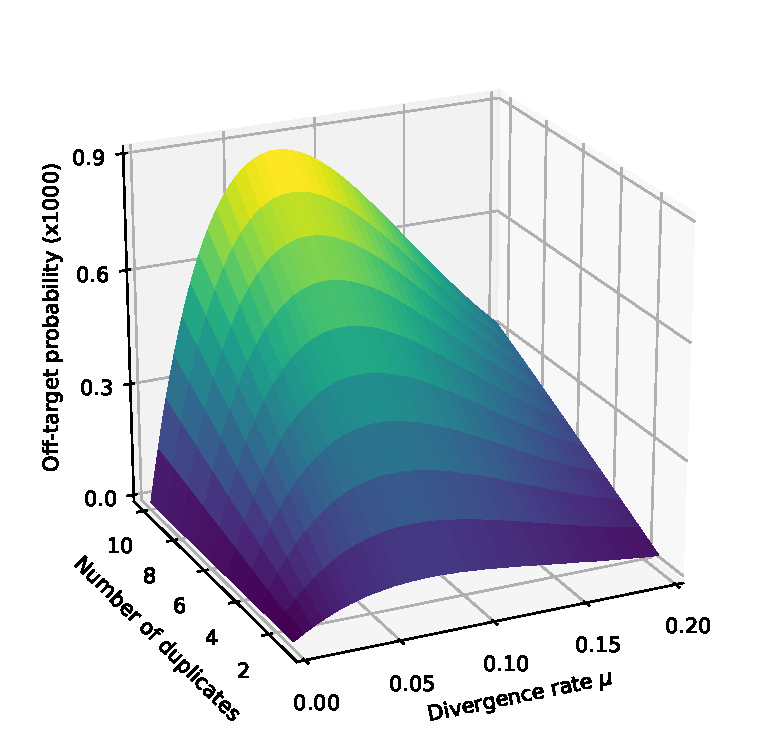
\includegraphics[scale=0.65]{curves_exact.pdf}
\caption{\textbf{Off target seeding probabilities (exact seeds).}
The curves show the probability that seeding is off target for exact seeds
of size $\gamma=17$ in reads of size $k=50$ nucleotides sequenced with an
error rate $p=0.01$. Each line shows a different number of duplicate
sequences $N$ from 1 to 10 and the x-axis shows the divergence rate $\mu$,
defined as the probability that a given duplicate differs from the target
at any given position.}
\label{fig:curves_exact}
\end{figure}

Fig.~\ref{fig:curves_exact} shows the result for a number of duplicates
$N$ from 1 to 10 and for a divergence rate $\mu$ from 0 to 0.20. The first
observation is that the probability that seeding is off target increases
with $N$. This is clearly visible from expression (\ref{eq:Poff}). This
can also be understood intuitively because the probability of null seeding
decreases when there are more potential candidates, and since the
probability of on-target seeding does not change, the probability of
off-target seeding must increase.

The second observation is that there exists a ``worst'' value of $\mu$
situated around 0.08. When $\mu$ is much smaller, the sequences of the
duplicates are close to that of the target so it is unlikely that the
candidate set contains one but not the other. When $\mu$ is much larger,
the sequences of the duplicates are far from that of the target and they
are unlikely to be in the candidate set. In expression (\ref{eq:Poff}),
the only term that depends on $\mu$ is $P(\overline{S}_0 \cap
\overline{S}_1)$, and it is obvious that the minimum of expression
(\ref{eq:Poff}) corresponds to the maximum of $P(\overline{S}_0 \cap
\overline{S}_1)$. This is why the worst value of $\mu$ is the same for
every $N$.

For comparison purposes, it is important to notice the order of magnitude
of the probabilities. Up to $N=3$ duplicates, off-target seeding has
probability lower than $10^{-4}$ and for $N=10$ duplicates the upper bound
is $3\cdot10^{-4}$. This sets a baseline to compare with more elaborate
seeding methods.


\section{Off-target skip seeds}

To compute the probability that the seeding process is off target when
using skip seeds, we observe that the logic of section~\ref{sec:offexact}
can be transposed with few modifications. In particular, the probability
can be computed through expression (\ref{eq:Poff}), where $S_0$ is the
event that the read has a \emph{skip} seed for the target and $S_1$ that
it has a \emph{skip} seed for the first duplicate.

We have already seen how to compute $P(\overline{S}_0)$ in
section~\ref{sec:example_skip}, we now need to find a way to compute
$P(\overline{S}_0 \cap \overline{S}_1)$ when using skip seeds.

\subsection{The skip dual encoding}

Once again, we start by recoding the reads in a specialized alphabet. We
define the skip-$n$ dual alphabet $\tilde{\mathcal{A}}_n = \{\square, |,
\Downarrow_0, \Downarrow_1, \Downarrow_2, \ldots, \Downarrow_n,
\downarrow^-_{/1}, \downarrow^-_{/2}, \ldots, \downarrow^+_{/1},
\downarrow^+_{/2}, \ldots\}$. The symbols $\square$, $|$,
$\downarrow^-_{/i}$ and $\downarrow^+_{/i}$ have the same meaning as in
the dual alphabet of section~\ref{sec:dual}. The symbols $\Downarrow_i$
indicate that both sequences have match length 0 and that the next
non-skipped position is $i$ nucleotides downstream.
 
Fig.~\ref{fig:skip_dual} shows the read from Fig.~\ref{fig:dual}
represented in the skip-3 dual encoding. It is important to note several
differences with Fig.~\ref{fig:dual}. The first is that the symbols
$\Downarrow_i$ are not always associated with double mismatches. For
instance, the symbol $\Downarrow_0$ on the right side of the read
corresponds to a mismatch for the $+$ sequence only. This happens whenever
the $+$ and the $-$ sequences are mismatched in the same interval between
non-skipped positions (the mismatches do not need to be on the same
nucleotide).

\begin{figure}[h]
\centering
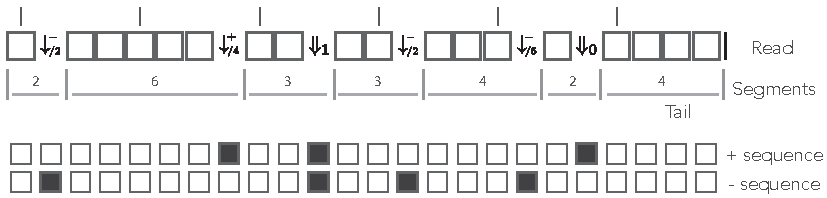
\includegraphics[scale=0.85]{sketch_skip_dual.pdf}
\caption{\textbf{Example skip dual encoding.}
The read of Fig.~\ref{fig:dual} is represented in the skip dual alphabet.
The vertical bars above the read indicate non-skipped positions. The
symbols $\downarrow_{/i}^-$ and $\downarrow_{/i}^+$ have the same meaning
as in the dual alphabet. The symbols $\Downarrow_i$ indicate that both
sequences have match length 0 and that the next non-skipped position is
located $i$ nucleotides downstream. Other features are as in
Fig.~\ref{fig:dual}.}
\label{fig:skip_dual}
\end{figure}

As in the case of the skip encoding, a fair amount of bookkeeping is
required to specify the weighted generating functions of interest.
We reuse the quantities $a+b+c+d=1$ and give them the same meaning as in
section~\ref{sec:dual}. For notational convenience, we define
\begin{eqnarray*}
N_i(z) &=& 1+z+\ldots+z^i, \\
W_j(z) &=& dz \cdot (az)^x \cdot \big( 1 + (az)^{n+1} + \ldots +
  (az)^{(n+1)m} \big), \\
  &\quad& \text{where } x = n-j \modulo{n+1},
  \text{ and } m = \left\lfloor
  \frac{\gamma-1-x}{n+1} \right\rfloor. \\
U_{i,j}(z) &=& dz \cdot (az)^x \cdot
  \big( 1 + (az)^{n+1} + \ldots + (az)^{(n+1)m} \big) +
\begin{cases}
  bz\cdot(az)^x \text{ if } j < y, \\
  0 \text{ otherwise}
\end{cases} \\
  &\quad& \text{where } x = -i-j-1 \modulo{n+1},
  y = n-i+1 \modulo{n+1}, \\
  &\quad& \text{and } m = \left\lfloor \frac{\gamma-1-i-x}{n+1}
    \right\rfloor, \\
V_{i,j}(z) &=& dz \cdot (az)^x \cdot
  \big( 1 + (az)^{n+1} + \ldots + (az)^{(n+1)m} \big) +
\begin{cases}
  cz\cdot(az)^x \text{ if } j \leq x, \\
  0 \text{ otherwise}
\end{cases} \\
  &\quad& \text{ where } x = -i-j-1 \modulo{n+1},
  m = \left\lfloor \frac{\gamma-1-i-x}{n+1} \right\rfloor.
\end{eqnarray*}

With these definitions, one can check that the expression of the transfer
matrix $\tilde{M}_n(z)$ is

\pagebreak

\begin{equation*}
\rotatebox{90}{$
\begin{blockarray}{cccccccccccc}
   & \scriptstyle{\Downarrow_0} & \scriptstyle{\Downarrow_1} &
   \ldots & \scriptstyle{\Downarrow_n} &
    \scriptstyle{\downarrow_{/1}^+} & 
    \ldots & \scriptstyle{\downarrow_{\gamma-1}^+} &
    \scriptstyle{\downarrow_{/1}^-} & \ldots &
    \scriptstyle{\downarrow_{/\gamma-1}^-} & \scriptstyle{|} \\
\begin{block}{c[ccccccccccc]}
\scriptstyle{\Downarrow_0} & W_0(z) & W_1(z) & \ldots & W_n(z) &
    r_0^+(z) & \ldots & r_{\gamma-2}^+(z) & r_0^-(z) & \ldots &
    r_{\gamma-2}^-(z) & F_{\gamma-1}(z) \\
\scriptstyle{\Downarrow_1} & z  & 0 & \ldots &
  0 & 0 & \ldots & 0 & 0 & \ldots & 0 & N_0(z) \\
\vdots & \vdots & \vdots & \ddots & \vdots & \vdots & \ddots &
  \vdots & \vdots & \ddots & \vdots & \vdots \\
\scriptstyle{\Downarrow_n} & z^n & 0 & \ldots &
  0 & 0 & \ldots & 0 & 0 & \ldots & 0 & N_{n-1}(z) \\
\scriptstyle{\downarrow_{/1}^+} & U_{1,0}(z) & U_{1,1}(z) & \ldots &
  U_{1,n}(z) & & & & & & & F_{\gamma-2}(z) \\
\vdots & \vdots & \vdots & \ddots & \vdots & & \tilde{A}(z) & & &
  \tilde{B}_n(z) & & \vdots \\
\scriptstyle{\downarrow_{/\gamma-1}^+} & U_{\gamma-1,0}(z) &
  U_{\gamma-1,1}(z) & \ldots & U_{\gamma-1,n}(z) & & & & & & & F_0(z) \\
\scriptstyle{\downarrow_{/1}^-} & V_{1,0}(z) & V_{1,1}(z) & \ldots &
    V_{1,n}(z) & & & & & & & F_{\gamma-2}(z) \\
\vdots & \vdots & \vdots & \ddots & \vdots & & \tilde{C}_n(z) &
  & & \tilde{D}(z) & & \vdots \\
\scriptstyle{\downarrow_{/\gamma-1}^-} & V_{\gamma-1,0}(z) &
    V_{\gamma-1,1}(z) & \ldots & V_{\gamma-1,n}(z) & & &
    & & & & F_0(z) \\
\scriptstyle{|} & 0 & 0 & \ldots & 0 & 0 & \ldots & 0 & 0 &
  \ldots & 0 & 0 \\
\end{block}
\end{blockarray}.
$}
\end{equation*}

\pagebreak

The matrices $\tilde{A}(z)$ and $\tilde{C}(z)$ in the expression of
$\tilde{M}_n(z)$ are the same as in section~\ref{sec:dual}. The matrices
$\tilde{B}_n(z)$ and $\tilde{C}_n(z)$ are defined as
\begin{equation*}
\tilde{B}_n(z) = 
\begin{blockarray}{cccccc}
   & \scriptstyle{\downarrow_{/1}^-} & \scriptstyle{\downarrow_{/2}^-} &
   \ldots & \scriptstyle{\downarrow_{/\gamma-2}^-} &
   \scriptstyle{\downarrow_{/\gamma-1}^-} \\
\begin{block}{c[ccccc]}
\scriptstyle{\downarrow_{/1}^+} & s_{1,1}(z) & s_{1,2}(z) &
    \ldots & s_{1,\gamma-2}(z) & s_{1,\gamma-1}(z) \\
\scriptstyle{\downarrow_{/2}^+} & s_{2,1}(z) & s_{2,2}(z) &
    \ldots & s_{2,\gamma-2}(z) & 0 \\
\vdots & \vdots & \vdots & \ddots & \vdots & \vdots \\
\scriptstyle{\downarrow_{/\gamma-2}^+} & s_{\gamma-2,1}(z) &
    s_{\gamma-2,2}(z) & \ldots & 0 & 0 \\
\scriptstyle{\downarrow_{/\gamma-1}^+} & s_{\gamma-1,1}(z) & 0 &
    \ldots & 0 & 0 \\
\end{block}
\end{blockarray},
\end{equation*}
\begin{equation*}
\tilde{C}_n(z) = 
\begin{blockarray}{cccccc}
   & \scriptstyle{\downarrow_{/1}^+} & \scriptstyle{\downarrow_{/2}^+} &
    \ldots & \scriptstyle{\downarrow_{/\gamma-2}^+} &
    \scriptstyle{\downarrow_{/\gamma-1}^+} \\
\begin{block}{c[ccccc]}
\scriptstyle{\downarrow_{/1}^-} & t_{1,1}(z) & t_{1,2}(z) &
    \ldots & t_{1,\gamma-2}(z) & t_{1,\gamma-1}(z) \\
\scriptstyle{\downarrow_{/2}^-} & t_{2,1}(z) & t_{2,2}(z) &
    \ldots & t_{2,\gamma-2}(z) & 0 \\
\vdots & \vdots & \vdots & \ddots & \vdots & \vdots \\
\scriptstyle{\downarrow_{/\gamma-2}^-} & t_{\gamma-2,1}(z) &
    t_{\gamma-2,2}(z) & \ldots & 0 & 0 \\
\scriptstyle{\downarrow_{/\gamma-1}^-} & t_{\gamma-1,1}(z) &
    0 & \ldots & 0 & 0 \\
\end{block}
\end{blockarray},
\end{equation*}
with
\begin{eqnarray*}
s_{i,j} &=&
  \begin{cases}
  cz \cdot (az)^{x+j-1} &\text{ if } i+j+x \leq \gamma \\
  0                     &\text{ otherwise,}
  \end{cases} \\
t_{i,j} &=&
  \begin{cases}
  bz \cdot (az)^{x+j-1} &\text{ if } i+j+x \leq \gamma \\
  0                     &\text{ otherwise,}
  \end{cases} \\
  \text{where } x &=& -i \modulo{n+1}, \text{ in both cases.} \\
\end{eqnarray*}

The computation is performed exactly as described in
section~\ref{sec:dual}. We compute the successive powers of
$\tilde{M}_n(z)$ in the arithmetic of truncated polynomials and stop the
iterations using the same criterion. So there is no change other than the
definition of the transfer matrix.

\begin{remark}
Observe that when $n=0$ the matrix $\tilde{M}_n(z)$ is identical to the
matrix $\tilde{M}_0(z)$ of section~\ref{sec:dual}, again consistent with
the fact that exact seeds are skip-$0$ seeds. The same applies to
$\tilde{B}_n(z)$ and $\tilde{C}_n(z)$.
\end{remark}


% XXX The following algorithm works but it is not very useful    XXX
% XXX because it is substantially slower than the WGF method.    XXX
% XXX It has been used to check the accuracy of the calculations XXX
% XXX but there is no reason to put it in the manuscript.        XXX

%\begin{algorithm}[H]
%\label{alg:mcmcskip}
%\SetAlgoLined
%\KwResult {Sample a read at random. Return 1 if the read contains a
%good seed, otherwise return 0.}
%  $\lambda \leftarrow 0$ \Comment*[r]{Current read size.}
%  $s_+ \leftarrow 0$ \Comment*[r]{Current + match size.}
%  $s_- \leftarrow 0$ \Comment*[r]{Current - match size.}
%  \While {$\lambda < k$}{
%    $i \leftarrow geom(1-a)-1$
%                \Comment*[r]{Double-match nucleotides.}
%    \If {$i \geq k-\lambda$}{
%      $s_+ \leftarrow s_+ + k-\lambda$ \;
%      $s_- \leftarrow s_- + k-\lambda$ \;
%      break \;
%    }
%    $s_+ \leftarrow s_+ + i$ \;
%    $s_- \leftarrow s_- + i$ \;
%    \If {$s_+ \geq \gamma$ or $s_- \geq \gamma$}{
%      return 1 \;
%    }
%    $\lambda \leftarrow \lambda + i+1$ \;
%    $r \leftarrow rand(0,1-a)$
%                \Comment*[r]{Uniform random number.}
%    \uIf {$r < b$}{
%      $s_+ \leftarrow s_++1$ \;
%      $s_- \leftarrow -(-\lambda \mod n+1)$ \;
%    }\uElseIf{$r < b+c$}{
%      $s_+ \leftarrow -(-\lambda \mod n+1)$ \;
%      $s_- \leftarrow s_-+1$ \;
%    }\Else{
%      $s_+ \leftarrow -(-\lambda \mod n+1)$ \;
%      $s_- \leftarrow -(-\lambda \mod n+1)$ \;
%    }
%}
%\eIf {$s_+ \geq \gamma$ or $s_- \geq \gamma$}{
%  return 1 \;
%}{
%  return 0 \;
%}
%\end{algorithm}


\subsection{Illustration}
\label{sec:illskipdual}

We illustrate the strategy delineated above Using the same settings as in
section~\ref{sec:illdual} ($k=50$, $p=0.01$ and $\gamma=17$), except that
we use skip-9 seeds instead of exact seeds.

\begin{figure}[h]
\centering
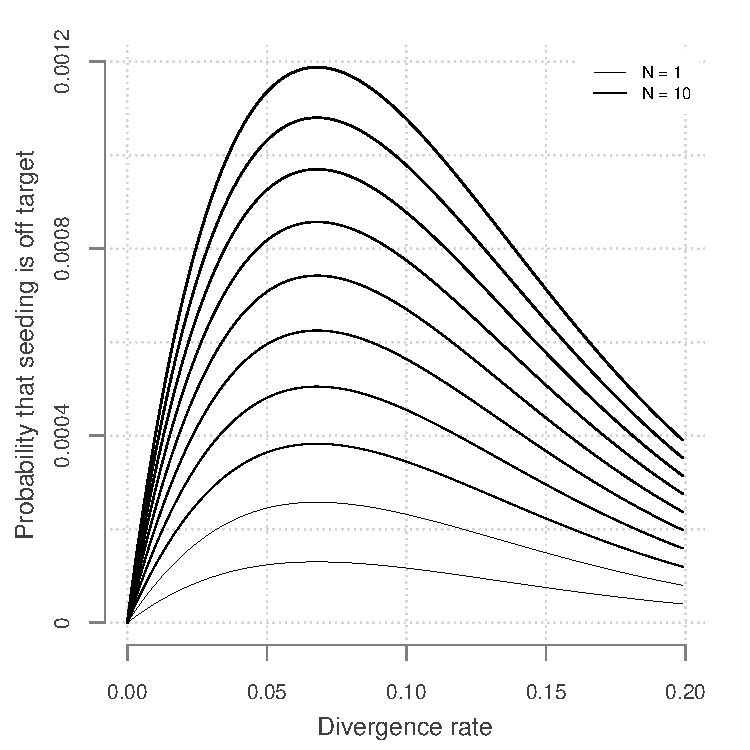
\includegraphics[scale=0.65]{curves_skip.pdf}
\caption{\textbf{Off target seeding probabilities (skip seeds).}
The curves show the probability that seeding is off target for skip-9
seeds of size $\gamma=17$. Read size and error rate are the same as in
Fig.~\ref{fig:curves_exact}, \textit{i.e.} $k=50$ and $p=0.01$. Each line
shows a different number of duplicate sequences $N$ from 1 to 10 and the
x-axis shows the divergence rate $\mu$, defined as the probability that a
given duplicate differs from the target at any given position.}
\label{fig:curves_skip}
\end{figure}

Fig.~\ref{fig:curves_skip} shows the result for a number of duplicates $N$
from 1 to 10 and for a divergence rate $\mu$ from 0 to 0.20. The curves
have the same general aspect as those of Fig.~\ref{fig:curves_exact}. The
probability that seeding is off target increases with $N$. There is again
a  worst value of $\mu$, because the maximum of $P(\overline{S}_0 \cap
\overline{S}_1)$ minimizes expression (\ref{eq:Poff}) for every value of
$N$. But the value is different from that of Fig.~\ref{fig:curves_exact}
because $P(\overline{S}_0 \cap \overline{S}_1)$ is computed for skip-9
seeds instead of exact seeds (here the worst value of $\mu$ is
approximately 0.07).

Importantly, Fig.~\ref{fig:curves_skip} reveals that skipping 9
nucleotides increases the chances that seeding is off target by a factor
approximately 4 (compare with Fig.~\ref{fig:curves_exact}). It is not
obvious why this should be the case: skip seeds reduce the probability of
on-target seeding (skipping positions implies fewer on-target seeds) but
increase the probability of null seeding (skipping positions implies fewer
seeds overall). So the net effect on off-target seeding is not intuitive.

And indeed, there are cases that skip seeds are \emph{less} prone to
off-target seeding than exact seeds. This is the case for instance when
$p=0.1$, where the ranking is inverted for the whole range of values
considered in Fig.~\ref{fig:curves_skip}.

This information is critical for choosing the best seeding strategy. The
off-target seeding probability is not the only criterion, though. Equally
important considerations are the probability of on-target seeding and the
computational resources required to implement a particular seeding
strategy. The benefit of a theory to compute seeding probabilities is to
have access to this knowledge.


\section{Off-target MEM seeds}

MEM seeds are substantially more complex than exact seeds and skip seeds
because we need to take into account all the duplicates in the
combinatorial construction.


\subsection{Hard and soft masking}

We first introduce two important notions that will be the key of
understanding the behavior of MEM seeds.

\begin{definition}
At a given position of the read, a duplicate is a \emph{hard mask} if its
match length on the left side is strictly longer than the match length
of the target. A duplicate is a \emph{soft mask} if it has the same match
length as the target.
\end{definition}

Fig.~\ref{fig:hard_vs_soft_masks} gives a graphical intuition of hard and
soft masks. It is important to bear in mind that hard and soft masks
depend on the position of interest: a sequence can be a mask at the left
end of the read and not at the right end, or the opposite.

\begin{figure}[h]
\centering
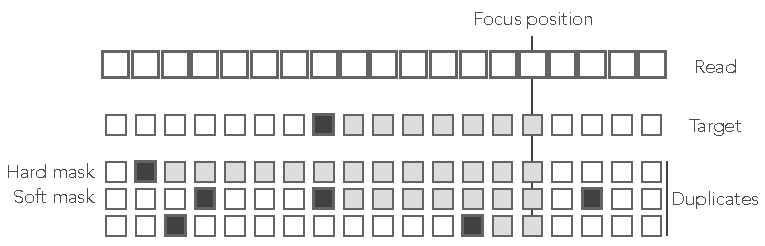
\includegraphics[scale=0.85]{hard_vs_soft_masks.pdf}
\caption{\textbf{Example of hard and soft masks.}
Genomic sequences are shown below a read where open squares represent
nucleotides. In the sequences, the open squares represent matches and the
closed squares represent mismatches. The nucleotides contributing to the
match length are represented as grey boxes. At the focus position, the
match length of the target is 7. The first duplicate is a hard mask
because its match length is $13>7$. The second duplicate is a soft mask
because its match length is 7, as the target. The third duplicate is not
a mask because its match length is $2<7$.}
\label{fig:hard_vs_soft_masks}
\end{figure}

Hard and soft masks explain the counter-intuitive properties of MEM seeds.
For instance, in Fig.~\ref{fig:full_masking_example} the target cannot be
discovered because every nucleotide of the read has a hard mask. In
Fig.~\ref{fig:short_vs_long}, the target could be discovered if the read
were shorter because a hard mask would turn into a soft one.

From the definition, we see that the last nucleotide of every strict
on-target MEM seed is always unmasked. Conversely, an unmasked nucleotide
always belongs to exactly one strict on-target MEM (not necessarily a seed
because the size of the MEM can be less than $\gamma$). Also, the last
nucleotide of every shared on-target MEM seed is always soft-masked, but a
soft-masked nucleotide does not always belong to a shared on-target MEM.

Since hard and soft masks inform us about the positions of on-target
MEM seeds, we construct an alphabet that encodes the masking status of the
nucleotides.

\subsection{The MEM alphabet}

As before, we recode the reads as sequences of letters from a specialized
alphabet called the MEM alphabet $\mathring{\mathcal{A}} = \{\square, |,
\uparrow_{/1}, \uparrow_{/2}, \uparrow_{/3} \ldots, \downarrow_{/0},
\downarrow_{/1}, \downarrow_{/2}, \ldots\}$.

The symbols $\downarrow_{/m}$ indicate that the nucleotide is a sequencing
error and $m \geq 0$ is the number of duplicates that \emph{match} the
nucleotide. Since a sequencing error is always a mismatch against the
target, the symbol $\downarrow_{/0}$ indicates that the nucleotide is a
mismatch against \emph{every} sequence. The symbols $\uparrow_{/i}$
indicate a change in masking status: the nucleotide is not masked but the
previous is --- this happens when all the duplicates fail to extend beyond
this position. The index $i \geq 1$ is the number of nucleotides since the
last mismatch or since the beginning of the read. All the other
nucleotides are represented by the symbol $\square$ and the symbol $|$ is
appended to the end of the read as usual.

Note that in the symbols $\downarrow_{/m}$ and $\uparrow_{/i}$, the
numbers $m$ and $i$ have different meanings. In the symbol
$\downarrow_{/m}$, the index $m$ is a number of sequences ($0 \leq m \leq
N$ where $N$ is the number of duplicates); in the symbol $\uparrow_{/i}$,
the index $i$ is a number of nucleotides. Fig.~\ref{fig:sketch_extended}
shows the encoding of a read in the MEM alphabet.

\begin{figure}[h]
\centering
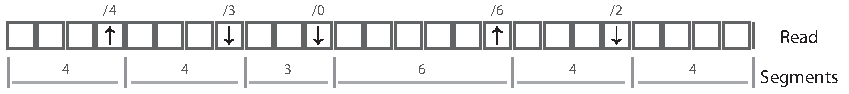
\includegraphics[scale=.84]{sketch_extended.pdf}
\caption{\textbf{The MEM encoding}.
The read of Fig.~\ref{fig:MEM_example} is represented in the MEM alphabet.
The arrows departing from the numbers help understand their meaning. The
symbol $\downarrow_{/m}$ is indexed by the number $m$ of locations that
match the nucleotide. The symbol $\uparrow_{/i}$ is indexed by the number
$i$ of nucleotides from the last error or from the beginning of the read.
The grey squares in the symbolic sequences represent MEM seed matches.
Other features are as in Fig.~\ref{fig:dual}.}
\label{fig:sketch_extended}
\end{figure}

The MEM alphabet captures the masking status of the nucleotide: the symbol
$\downarrow_{/m}$ indicates that the nucleotide has $m$ hard masks and
$N-m$ soft masks. The symbols $\uparrow_{/i}$ indicate that the nucleotide
is unmasked and that the previous nucleotide is masked.

In the MEM alphabet, strict on-target MEM seeds are the longest stretches
of symbols containing some symbol $\uparrow_{/i}$ and not containing any
symbol $\downarrow_{/m}$. Indeed, such a stretch is a match for the target
because it does not contain any symbol $\downarrow_{/m}$, it only matches
the target because it contains at least one unmasked nucleotide (marked by
$\uparrow_{/i}$), and it cannot be extended because it is flanked by
sequencing errors (symbols $\downarrow_{/m}$) or by the ends of the reads.
Note that there is exactly one symbol $\uparrow_{/i}$ per strict on-target
MEM seed, and therefore two symbols $\uparrow_{/i}$ must be separated by
at least one symbol $\downarrow_{/m}$.

Shared on-target MEM seeds are the longest stretches of symbols $\square$
flanked by $\downarrow_{/0}$, or by the ends of the read. Indeed, such a
stretch is a MEM seed because it matches the target and it cannot be
extended ($\downarrow_{/0}$ is a mismatch against every sequence). Also,
it cannot be a strict on-target MEM seed because it does not contain any
$\uparrow_{/i}$ symbol, so it must be a shared on-target MEM seed.

As before, the read is converted from a sequence of symbols to a sequence
of segments that consist of 0 or more symbols $\square$ followed by a
terminator. We then specify the weighted generating functions of those
segments and fill the transfer matrix $\mathring{M}_N(z)$ of the reads that
do not contain an on-target MEM seed. We introduce the terms of the matrix
by increasing order of complexity.


\subsection{Segments following $\uparrow_{/i}$}

A segment terminated by $\uparrow_{/i}$ is the beginning of a strict
on-target MEM of size at least $i$. The MEM reaches the next sequencing
error or the end of the read, so the number of symbols $\square$ in the
next segment must be at most $\gamma-i-1$ and it must be terminated by a
$\downarrow_{/m}$ symbol or by the tail terminator $|$.

The following definition will simplify the notations.

\begin{definition}
The probability that a symbol is $\downarrow_{/m}$ given that the
nucleotide is a read error is
\begin{equation}
\label{eq:omega}
\omega_m = {N \choose m} \big(1 - \mu/3\big)^{N-m} \big(\mu/3\big)^m.
\end{equation}
\end{definition}

The expression for $\omega_m$ is exact: if the nucleotide is an error,
the symbol is $\downarrow_{/m}$ for some $m$ between 0 and $N$. Each
duplicate is a match with probability $\mu/3$, so $m$ has a Binomial
distribution with parameters $(N, \mu/3)$.

On this segment, the matches between the read and the duplicates are
irrelevant, so the weighted generating function of a symbol $\square$ is
simply $qz$ (recall that $p = 1-q$ is the probability of a sequencing
error). The weighted generating function of the terminator
$\downarrow_{/m}$ is $\omega_m pz$, so the weighted generating function of
the $\downarrow_{/m}$ segments following $\uparrow_{/i}$ is
\begin{equation}
\label{eq:D}
D_{i,m}(z) = \omega_m pz \sum_{j=0}^{\gamma-i-1} (qz)^j.
\end{equation}

And the weighted generating function of the tail segments following
$\uparrow_{/i}$ is
\begin{equation}
\label{eq:E}
E_i(z) = \sum_{j=0}^{\gamma-i-1} (qz)^j.
\end{equation}


\subsection{Segments following $\downarrow_{/m}$}

The symbol $\downarrow_{/m}$ signifies that the nucleotide has $m$ hard
masks and $N-m$ soft masks. If all the masks vanish before the first read
error, the next terminator will be a symbol $\uparrow_{/j}$, otherwise it
will be the symbol $|$ or a symbol $\downarrow_{/m}$. We separate the
cases based on the terminator of the segment.

\subsubsection*{Case 1: the terminator is $\uparrow_{/j}$}

\begin{definition}
The probability that a given duplicate contains a mismatch in a sequence
of $j$ error-free nucleotides is
\begin{equation}
\label{eq:xi}
\xi_j = 1-(1-\mu)^j.
\end{equation}
This is the probability that a hard or soft mask vanishes within $j$
correct nucleotides.
\end{definition}

The expression for $\xi_j$ is exact: every nucleotide of the duplicate
differs from the target with probability $\mu$. In the absence of
sequencing errors, this is also the probability that a nucleotide of the
duplicate differs from the read. Given that there is no error, the
probability that $j$ nucleotides in a row are identical to the read is
thus $(1-\mu)^j$ and the probability that at least one of them is
different is the complement $1-(1-\mu)^j$.

With this notation, the probability that at least one of $N$ masks
survives a sequence of $j$ error-free nucleotides is thus $1-(\xi_j)^N$,
and the probability that there remains a mask at the $j-1$-th but not at
the $j$-th error-free nucleotide is $(\xi_j)^N - (\xi_{j-1})^N$. From this
we conclude that the weighted generating function of the segments
terminated by $\uparrow_{/j}$ following a segment terminated by
$\downarrow_{/m}$ is
\begin{equation}
\label{eq:B}
B_j(z) = \Big( (\xi_j)^N-(\xi_{j-1})^N \Big) (qz)^j.
\end{equation}

The fact that the reads have no on-target seeds imposes $j < \gamma$. Also
note that this expression is the same for all symbols $\downarrow_{/m}$
(it does not depend on $m$).

\subsubsection*{Case 2a: the terminator $|$ comes before the $\gamma$-th
nucleotide}

In this case there can be no on-target seed because the read finishes too
early. However, we must enforce the condition that at least one of the $N$
masks survives until the end, otherwise the segment would be terminated by
one of the symbols $\uparrow_{/j}$. The weighted generating function is
\begin{equation*}
\sum_{i=0}^{\gamma-1} \Big(1 - (\xi_i)^N \Big) (qz)^i.
\end{equation*}

\subsubsection*{Case 2b: the terminator $|$ comes after the $\gamma$-th
nucleotide}

In this case, the soft masks do not hide the target. Even if a duplicate
survives until the end of the read, there will be an on-target seed
(shared in this case). To exclude on-target seeds, we must enforce the
condition that at least one hard mask survives until the end of the
segment (which is impossible if $m = 0$). The weighted generating function
is
\begin{equation*}
\sum_{i=\gamma}^\infty \Big(1 - (\xi_i)^m \Big) (qz)^i.
\end{equation*}

Summing the expressions from cases 2a and 2b, we find that the
weighted generating function of the tail following $\downarrow_{/m}$ is
\begin{equation}
\label{eq:C}
C_m(z) =
\sum_{i=0}^{\gamma-1} \Big(1 - (\xi_i)^N \Big) (qz)^i +
  \sum_{i=\gamma}^\infty \Big(1 - (\xi_i)^m \Big) (qz)^i.
\end{equation}

\subsubsection*{Case 3a: the terminator $\downarrow_{/n}$ comes before the
$\gamma$-th nucleotide}

In this case, there can be no on-target seed and we must only exclude the
terminators $\uparrow_{/j}$. As we have seen above, this implies that at
least one of the $N$ masks survives until the terminator. For a read of
size $j+1$, this occurs with probability $1-(\xi_j)^N$. Including the
terminator and summing over $j+1 \leq \gamma$, we see that the weighted
generating function is
\begin{equation}
\omega_n pz \sum_{j=0}^{\gamma-1} \Big(1 - (\xi_j)^N \Big) (qz)^j.
\end{equation}

\subsubsection*{Case 3b: the terminator $\downarrow_{/n}$ comes after the
$\gamma$-th nucleotide}

This case is by far the most convoluted. Since the segment contains at
least $\gamma$ error-free nucleotides, we must enforce the condition that
it does not contain an on-target seed. This will be the case if any of the
two following conditions is validated: $i)$ at least one hard mask covers
all the error-free nucleotides, or $ii)$ all the hard masks vanish but at
least one soft mask covers the whole segment (including the terminator).

The two conditions are mutually exclusive by construction. They are
graphically represented in the diagram below. The left panel corresponds
to case $i)$ and the right panel to case $ii)$. The top row represents the
target, and the bottom rows represent duplicates (using the same symbols
as in Fig.~\ref{fig:sketch_extended}).
\begin{inset}

\includegraphics{masks.pdf}
\end{inset}

Whenever a hard mask (here the first duplicate) covers the nucleotides as
shown by the grey squres in the left panel, there can be no on-target
seed. The positions marked with a question mark are irrelevant, they
cannot change the fact that there is no on-target MEM seed. If the hard
masks vanish, as in the right panel, then we need to look at the soft
masks. If a soft mask covers the whole segment as indicated by the grey
squares, then there can be no on-target seed. In all other cases there is
an on-target MEM seed.

For a segment of size $j+1$, condition $i)$ has probability $\big(1 -
(\xi_j)^m \big)$. Summing over $j+1 > \gamma$ and including the
terminator, we see that the associated weighted generating function is
\begin{equation*}
\omega_n pz \sum_{j=\gamma}^\infty \Big(1 - (\xi_j)^m \Big) (qz)^j.
\end{equation*}

Condition $ii)$ is more convoluted, so we introduce some further
notations to solve this sub-case.
\begin{definition}
The probability that a given duplicate sequence contains a mismatch in a
sequence of $j$ error-free nucleotides followed by an error is
\begin{equation}
\label{eq:eta}
\eta_j = 1-(1-\mu)^j\mu/3.
\end{equation}
This is the probability that a hard or soft mask vanishes within $j$
correct nucleotides followed by a sequencing error.
\end{definition}

The expression for $\eta_j$ is exact: the probability that there are $j$
matches between the duplicate and the target is $(1-\mu)^j$. If there are
no sequencing errors, this is also the probability that there are $j$
matches between the duplicate and the read. The probability that the
duplicate matches the subsequent error is $\mu/3$, so the probability
that there are $j+1$ matches including the sequencing error is
$(1-\mu)^j\mu/3$. Finally, the probability that there is a mismatch is the
complement $1-(1-\mu)^j\mu/3$.

Let us for now consider a segment of fixed size $j+1$. From expressions
(\ref{eq:xi}) and (\ref{eq:eta}), the probability of condition $ii)$ is
\begin{equation*}
(\xi_j)^m \Big(1 - (\eta_j)^{N-m} \Big),
\end{equation*}
but we need to break up this term among all the possible terminators
$\downarrow_{/n}$ ($0 \leq n \leq N$) in order to fill the different
entries of the transfer matrix. For this, we split this term in the number
of soft masks that run until and including the terminator. From expression
(\ref{eq:eta}), the probability that there are $r \geq 1$ such soft masks
is
\begin{equation}
\label{eq:softmasks_r}
{N-m \choose r} (1 - \eta_j)^r (\eta_j)^{N-m-r}.
\end{equation}

For now we consider $r$ fixed; we will compute the marginal probability at
the final stage. By construction, each of those $r$ soft masks matches the
terminator, so the total number of matches is $r$ plus the number of
sequences that also match the terminator, among the remaining $N-m-r$ soft
masks and the $m$ hard masks.

Let us start with the $m$ hard masks. The probability that each of them
matches the terminator is simply $\mu/3$.

The case of the $N-m-r$ soft masks is more complicated because they can
vanish precisely on the terminator --- recall that in case $ii$) all the
hard masks are assumed to vanish before. If the soft mask failed within
the first $j$ nucleotides, then the $j+1$-th nucleotide can be anything
and it will match the terminator with probability $\mu/3$. But if the soft
mask survived the first $j$ nucleotides, then it \emph{must} fail on the
$j+1$-th and it cannot match the terminator. From expressions
(\ref{eq:xi}) and (\ref{eq:eta}), the probability that a given soft mask
fails within the first $j$ nucleotides is $\xi_j/\eta_j$ --- this is the
conditional probability that it fails within the first $j$ nucleotides
given that it fails within the segment. Finally the probability that such
a soft mask matches the terminator is $\mu/3 \cdot \xi_j / \eta_j$.

Summing the contributions of the hard masks ($m$ in total, each matching
the terminator with probability $\mu/3$) and of the soft masks ($N-m-r$ in
total, each matching the terminator with probability
$\mu/3\cdot\xi_j/\eta_j$), the probability that the total number of
matches is $n-r$ appears as the convolution product
\begin{eqnarray*}
\frac{(\mu/3)^{n-r}(1-\mu/3)^{N-n}}{(\eta_j)^{N-m-r}}
&\psi_{j,m,n,r}&, \\
\text{where }
&\psi_{j,m,n,r}& = \sum_{q \geq 0}{m \choose q}{N-m-r \choose n-r-q}
(\xi_j)^{n-r-q}.
\end{eqnarray*}

Finally, we need to compute the marginal probability over the number $r$
of soft masks that survive until the end of the read. Multiplying by the
probability of $r$ from expression (\ref{eq:softmasks_r}) and summing over
$r \geq 1$, the probability that $n$ duplicate sequences match the
terminator appears as
\begin{eqnarray*}
&\;& \sum_{r\geq1} {N-m \choose r}
(1 - \eta_j)^r (\mu/3)^{n-r} (1-\mu/3)^{N-n} \psi_{j,m,n,r} \\
&=& (\mu/3)^n(1-\mu/3)^{N-n} \sum_{r\geq1} {N-m \choose r}
  (1 - \mu)^{rj} \psi_{j,m,n,r} \\
&=& \omega_n \cdot \zeta_{j,m,n},
\end{eqnarray*}
where
\begin{equation}
\label{eq:zeta}
\zeta_{j,m,n} = \sum_{r\geq1} {N-m \choose r}
(1-\mu)^{rj} \psi_{j,m,n,r} \bigg/ {N \choose n}.
\end{equation}

This is the probability that the terminator is the symbol
$\downarrow_{/n}$ given that the segment has size $j+1 > \gamma$, that
the first sequencing error occurs on the last nucleotide, that the
preceding terminator was $\downarrow_{/m}$ and that the $m$ hard masks
fail before the end of the segment.

Summing the terms from case 3a and from case 3b, we find that the weighted
generating function of the $\downarrow_{/n}$ segments following
$\downarrow_{/m}$ is
\begin{equation}
\begin{split}
\label{eq:A}
A_{m,n}(z) =
&\omega_n pz \sum_{j=0}^{\gamma-1} \Big(1 - (\xi_j)^N \Big)
  (qz)^j \\
+ &\omega_n pz \sum_{j=\gamma}^\infty \Big(1 - (\xi_j)^m \cdot
(1- \zeta_{j,m,n}) \Big) (qz)^j.
\end{split}
\end{equation}

\subsection{Expression of $\mathring{M}_N(z)$}
\label{sec:expression_of_M}

Collecting and arranging the results above, we can verify that the final
expression of the transfer matrix $\mathring{M}_N(z)$ is
\begin{equation*}
\begin{blockarray}{cccccccc}
   & \dn{0} & \ldots & \dn{N} & \up{1} & \ldots & \up{\gamma-1} & \nd \\
\begin{block}{c[ccccccc]}
\dn{0} & A_{0,0}(z) & \ldots & A_{0,N}(z) & B_1(z) & \ldots &
    B_{\gamma-1}(z) & C_0(z) \\
\vdots & \vdots & \ddots & \vdots & \vdots & \ddots &
    \vdots & \vdots \\
\dn{N} & A_{N,0}(z) & \ldots & A_{N,N}(z) & B_1(z) & \ldots &
    B_{\gamma-1}(z) & C_N(z) \\
\up{1} & D_{1,0}(z) & \ldots & D_{1,N}(z) & 0 & \ldots & 0 & E_1(z) \\
\vdots & \vdots & \ddots & \vdots & \vdots & \ddots &
    \vdots & \vdots \\
\up{\gamma-1} & D_{\gamma-1,0}(z) & \ldots & D_{\gamma-1,N}(z) & 0 &
  \ldots & 0 & E_{\gamma-1}(z) \\
\nd & 0 & \ldots & 0 & 0 & \ldots & 0 & 0 \\
\end{block}
\end{blockarray}
\end{equation*}
where
\begin{equation}
\tag{\ref{eq:A}}
\begin{split}
A_{m,n}(z) =
&\omega_n pz \sum_{i=0}^{\gamma-1} \Big(1 - (\xi_i)^N \Big) (qz)^i \\
+ &\omega_n pz \sum_{i=\gamma}^\infty \Big(1 - (\xi_i)^m \cdot
(1- \zeta_{i,m,n}) \Big) (qz)^i 
\end{split}
\end{equation}
\begin{gather}
\tag{\ref{eq:B}}
B_i(z) = \Big( (\xi_i)^N-(\xi_{i-1})^N \Big) (qz)^i \\
\tag{\ref{eq:C}}
C_m(z) =
\sum_{i=0}^{\gamma-1} \Big(1 - (\xi_i)^N \Big) (qz)^i +
  \sum_{i=\gamma}^\infty \Big(1 - (\xi_i)^m \Big) (qz)^i \\
\tag{\ref{eq:D}}
D_{j,m}(z) = \omega_m pz \sum_{i=0}^{\gamma-j-1} (qz)^i \\
\tag{\ref{eq:E}}
E_j(z) = \sum_{i=0}^{\gamma-j-1} (qz)^i
\end{gather}
and where
\begin{gather}
\tag{\ref{eq:omega}}
\omega_m = {N \choose m} \big(1 - \mu/3\big)^{N-m} \big(\mu/3\big)^m \\
\tag{\ref{eq:xi}}
\xi_j = 1-(1-\mu)^j \\
\tag{\ref{eq:eta}}
\eta_j = 1-(1-\mu)^j\mu/3 \\
\tag{\ref{eq:zeta}}
\zeta_{j,m,n} = \sum_{r\geq1} {N-m \choose r}
(1-\mu)^{rj} \psi_{j,m,n,r} \bigg/ {N \choose n} \\
\notag
\psi_{j,m,n,r} = \sum_{q \geq 0}{m \choose q}{N-m-r \choose n-r-q}
(\xi_j)^{n-r-q}.
\end{gather}

\begin{remark}
In the special case $N=0$, the transfer matrix simplifies to the extent
that we can compute the weighted generating function of the reads without
on-target MEM seed in closed form. The result is
\begin{equation}
\tag{\ref{eq:F}}
\frac{1+qz+\ldots+(qz)^{\gamma-1}}
  {1-pz \big(1+qz+\ldots+(qz)^{\gamma-1} \big)}.
\end{equation}

Expression (\ref{eq:F}) was shown in section~\ref{sec:example_exact} to be
the weighted generating function of reads without on-target exact seed.
This shows that when there are no duplicates, MEM seeds have exactly the
same properties as exact seeds.
\end{remark}

\subsection{Computing MEM seeding probabilities}

The matrix $\mathring{M}_N(z)\cdot(I-\mathring{M}_N(z))^{-1}$ contains the
weighted generating functions of all the reads without on-target MEM
seeds. The term of interest, as usual, is the top right entry. Indeed,
every read can be prepended by $\downarrow_{/0}$ segments and only by
those, otherwise the read would start with fewer than $N$ soft masks.
Thus, reads without an on-target MEM seed are precisely the sequences of
segments that can be appended to the symbol $\downarrow_{/0}$ and that are
terminated by a tail.

To compute this term, we proceed as in section~\ref{sec:example_skip},
\textit{i.e.}, we compute the powers of $\mathring{M}_N(z)$ in the
arithmetic of truncated polynomials and we stop the iterations when the
terms are negligible. We bound the probability that the read contains more
than $e$ sequencing errors using the expression
\begin{equation*}
\tag{\ref{eq:bound}}
Pr(X \geq e) \leq \exp \left( (e-k)\log \frac{k-e}{k(1-p)} -e\log
\frac{e}{kp} \right),
\end{equation*}
but here not every segment contains an error. There cannot be two symbols
$\uparrow_{/j}$ in a row, so a read with $s+1$ segments must contain a
minimum number of sequencing errors which is $e=\lfloor{s/2\rfloor}$. As
before, we compute the powers of $\mathring{M}_N(z)$ until the upper bound
is less than a set fraction $\varepsilon$ of the current value of $a_k$.

If we call $M_0$ the event that the read contains an on-target MEM seed,
the method above gives us $P(\overline{M}_0)$. Calling $M_j$ the event
that the read contains a MEM seed for the $j$-th duplicate, we are
interested in the probability
\begin{equation*}
\tag{\ref{eq:pcomp}}
P\big(\overline{M}_0 \cap (M_1 \cup \ldots \cup M_N)\big) =
P(\overline{M}_0) - P\big(\overline{M}_0 \cap \overline{M}_1 \cap \ldots
\cap \overline{M}_N\big).
\end{equation*}

The key insight to compute $P\big(\overline{M}_0 \cap \overline{M}_1 \cap
\ldots \cap \overline{M}_N\big)$ is to realize that there is some MEM
seed, on-target or not, if and only if the read contains a match of size
$\gamma$ or more for any of the $N+1$ sequences. Therefore, this
probability is the same as the term $P\big(\overline{S}_0 \cap
\overline{S}_1 \cap \ldots \cap \overline{S}_N\big)$ computed in
section~\ref{sec:offexact}.

In conclusion, the probability that the MEM seeding process is off target
is
\begin{equation}
\label{eq:PMEM}
P(\overline{M}_0) - P(\overline{S}_0) \cdot \left( \frac{P(\overline{S}_0
\cap \overline{S}_1)}{P(\overline{S}_0)} \right)^N,
\end{equation}
where $P(\overline{M}_0)$ is computed using $\mathring{M}_N(z)$ as
explained in this section, $P(\overline{S}_0)$ is computed using a
recursive equation as explained in section~\ref{sec:example_exact}, and
$P(\overline{S}_0\cap\overline{S}_1)$ is computed using $\tilde{M}_0(z)$
as explained in section~\ref{sec:dual}.

\subsection{Monte Carlo sampling}
\label{sec:montecarlo}

One potential difficulty in computing $P(\overline{M}_0)$ is that the
matrix $\mathring{M}_N(z)$ has dimension $(N+\gamma+1) \times
(N+\gamma+1)$. The problem can become computationally intractable because
$N$ can be very large. For instance, the sequences called \emph{Alu} have
more than one million duplicates in the human genome. There is no hope to
compute the powers of $\mathring{M}_N(z)$ in these conditions and we need
an alternative method.

The symbolic representation as MEM segments can be used to design an
efficient method to sample reads. Instead of generating the nucleotides of
the $N+1$ sequences one by one, one can generate a single sequence of
segments. Since the number of segment does not depend on $N$, we can
obtain a fast Monte Carlo method to sample millions of reads and count the
proportion that contain an on-target MEM seed.

The principle is to proceed in cycles of two steps. We first sample the
position of the next sequencing error, which gives the position of the
next symbol $\downarrow_{/m}$, where $m$ will be determined at a later
stage. The second step is to determine whether there is a symbol
$\uparrow_{/j}$ before that. For this we sample the number of masks that
vanish before the symbol $\downarrow_{/m}$. If they all vanish, the read
contains an on-target MEM seed, provided the next read error is at a
distance greater than $\gamma$. Otherwise, we sample the number $m$ of
hard masks at the sequencing error, and the process is repeated until we
generate an on-target MEM seed, or until the read has size $k$ or greater
(in which case it has no on-target MEM seed).

The method is summarized in algorithm~\ref{alg:mcmc} below. It requires
efficient algorithms to sample from the geometric and from the binomial
distributions. Sampling from a geometric distribution can be done by
computing the logarithm of a uniform $(0,1)$ random variable. Sampling
from a binomial distribution can be done by the method of
Kachitvichyanukul and Schmeiser~\cite{kachitvichyanukul1988binomial}.
Most importantly, the number of duplicates $N$ has little influence on
the running speed of algorithm~\ref{alg:mcmc}.

\begin{algorithm}[H]
\SetKwInOut{Parameter}{Parameter}
\label{alg:mcmc}
\SetAlgoLined
\Parameter {$k$ is the size of the reads.}
\Parameter {$p$ is the error rate of the sequencer (substitutions only).}
\Parameter {$N$ is the number of duplicates.}
\Parameter {$\mu$ is the nucleotide-wise probability that duplicates
differ.}
\KwResult {Sample a read at random. Return 1 if the read contains a
good MEM seed, otherwise return 0.}
  $\lambda \leftarrow 0$ \Comment*[r]{Current read size.}
  $m \leftarrow 0$ \Comment*[r]{Current number of hard masks.}
  \While {$\lambda < k$}{
    $i \leftarrow geom(p)-1$ \Comment*[r]{Error-free nucleotides.}
    \eIf {$i \geq k-\lambda$}{
      \eIf{$k-\lambda < \gamma$} {
        return 0\; }{
        $h \leftarrow binom(m,(1-\mu)^{k-\lambda})$
            \Comment*[r]{Surviving hard masks.}
        return 1 if $h = 0$, otherwise return 0\; }
    }
    {
      $h \leftarrow binom(m,(1-\mu)^i)$
          \Comment*[r]{Surviving hard masks.}
      $s \leftarrow binom(N-m,(1-\mu)^i \mu/3)$
          \Comment*[r]{Surviving soft masks.}
      \eIf {$ i \geq \gamma$ and $h = 0$ and $s = 0$}{
        return 1\;}{
        $m \leftarrow s + binom(N-s, \mu/3)$\;
        $\lambda \leftarrow \lambda + i+1$\;}
    }
 }
\end{algorithm}

Algorithm~\ref{alg:mcmc} is an important result. It gives a compact
solution to the problem of estimating the probability that a read can be
mapped when using MEM seeds. The algorithm is also much faster than the
naive approach of sampling every nucleotide of every sequence, because it
is equivalent to sampling the nucleotide sequence of \emph{all} the
duplicates.

\subsection{Illustration}
\label{sec:illmem}

We illustrate the strategy delineated above 
using the same settings as in section~\ref{sec:illdual} ($k=50$, $p=0.01$
and $\gamma=17$), except that we replace exact seed by MEM seeds.

\begin{figure}[h]
\centering
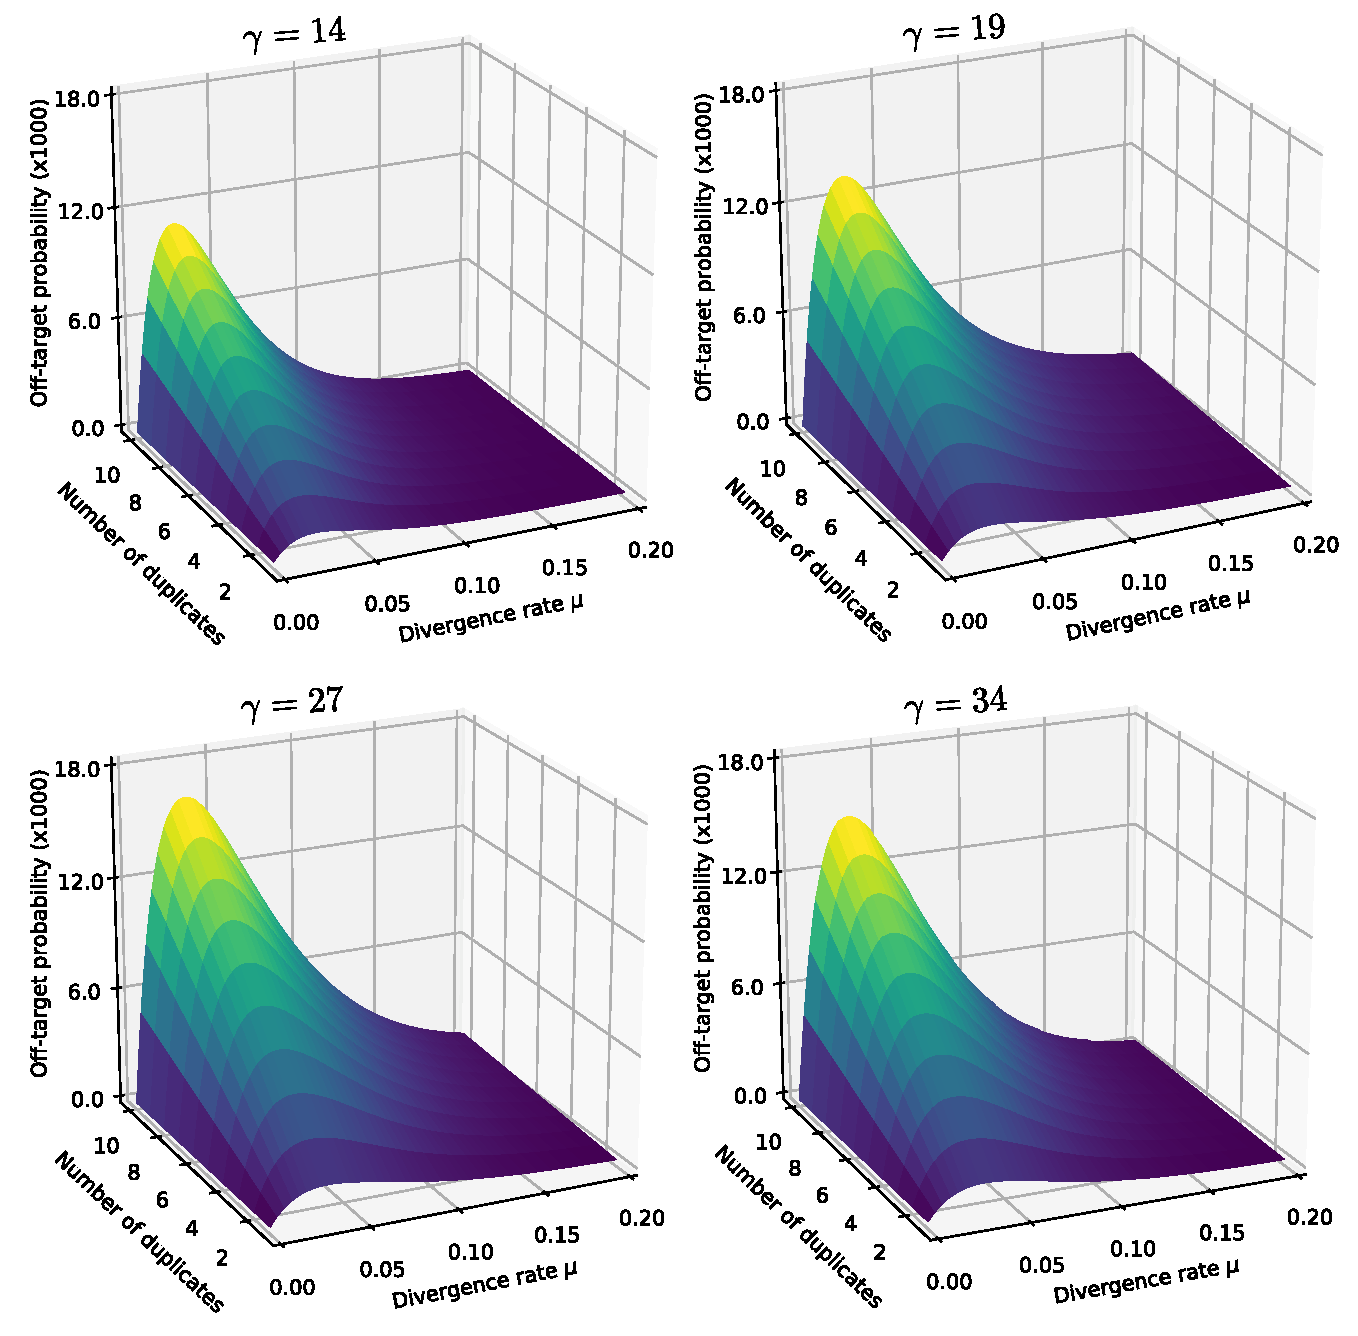
\includegraphics[scale=0.65]{curves_mem.pdf}
\caption{\textbf{Off target seeding probabilities (MEM seeds).}
The curves show the probability that seeding is off target for MEM
seeds of minimum size $\gamma=17$. Read size and error rate are the same
as in Fig.~\ref{fig:curves_exact}, \textit{i.e.} $k=50$ and $p=0.01$. Each
line shows a different number of duplicate sequences $N$ from 1 to 10 and
the x-axis shows the divergence rate $\mu$, defined as the probability
that a given duplicate differs from the target at any given position.}
\label{fig:curves_mem}
\end{figure}

Fig.~\ref{fig:curves_mem} shows the result for a number of duplicates $N$
from 1 to 10 and for a divergence rate $\mu$ from 0 to 0.20. The curves
have the same general aspect as those of Fig.~\ref{fig:curves_exact}. The
probability that seeding is off target increases with $N$, as shown by
expression (\ref{eq:PMEM}).

There is again a  worst value of $\mu$ but it is much lower than the
previous two cases (here it is close to 0.026). In the case of MEM seeds,
it is not obvious why the same value of $\mu$ maximizes (\ref{eq:PMEM})
for all values of $N$ because both $P(\overline{M}_0)$ and
$P(\overline{S}_0 \cap \overline{S}_1)$ depend on $\mu$.

Fig.~\ref{fig:curves_mem} reveals that in this concrete case, MEM seeds
increase the chances that seeding is off target by a factor up to 40
compared to exact seeds (see Fig.~\ref{fig:curves_exact}). On this
criterion, MEM seeds are always inferior to exact seeds with the same
specifications. The reason is that every read triggering an off-target
seeding with exact seeds will also trigger an off-target seeding with MEM
seeds. Knowing that, it is still important to realize how large the
increase is in practice. MEM seeds tremendously simplify the seeding
process, but this comes at the cost of an increase in the false positive
rate. The methods presented here are thus very useful to balance the
risk when using MEM seeds.


\section{Random seeds}
\label{sec:random_seeds}

We have assumed throughout that seeds can match only the target or one of
its duplicates. In practice, seeds can match many random locations of the
genome and not just the target and the duplicates.

It is important for the validity of the theory that all the sequences that
have a seed are considered candidate locations (as long as the seed is
above the threshold $\gamma$). If not, the final estimates are biased. The
hope is that spurious matches are shorter than $\gamma$ so that they are
filtered out, but this is not always the case. And if they qualify as a
seed we need to verify the candidate location.

Such random hits can be problematic for two reasons: First, the time spent
verifying them is wasted. Second, they can cause false positives.
Fortunately, both issues can be addressed.

To save time during the alignment phase, we can prioritize the seeds so
that the best hit is likely to be discovered first, allowing us to bail
out from other alignments as early as possible. We can even bound the
maximum quality of some candidates so that the alignment can be skipped
altogether. These considerations depend on the implementation of the
mapper so we will not develop this further. What matters is that random
hits do not impose a significant burden on the time needed to verify the
candidates.

The second issue is that random hits can generate false positives. Such
cases occur when seeding is null (meaning that there is no seed for the
target nor for its duplicates). Since the hits are not homologous to the
read, the alignment score is extreme, which makes it easy to detect.

Indeed, if the candidate location is random, mismatches occur with
probability 3/4. If it is the true location, mismatches occur with
probability $p$. We discard the seed because it is an automatic match of
size $\gamma$ (and possibly larger in the case of MEM seeds). Say that
there remain $L$ nucleotides and that $m$ of them are mismatches for the
candidate location. From Bayes formula, the probability that the location
is random given the number of mismatches is
\begin{equation}
\label{eq:bayes}
\frac{1}{1 + 4^L(p/3)^mq^{L-m}(1-\beta)/\beta},
\end{equation}
where $q=1-p$ and $\beta$ is the prior probability that the hit is
random.

The value of $\beta$ has little importance if $p$ is small. Say that
$p=0.01$ and that a read generates a hit in the genome such that 33
nucleotides need to be aligned after seeding. If the hit is random there
is a 99.99\% chance that at least 15 are mismatches. The denominator of
expression (\ref{eq:bayes}) is approximately $1 +
4.3\cdot10^{-18}(1-\beta)/\beta$. So unless $\beta < 10^{-17}$, the
support for the hypothesis that the hit is random is overwhelming.
Conversely, if the hit is not random, there is a 99.99\% chance that 4 or
fewer nucleotides are mismathes. In this case, the denominator is
approximately $1+6.8\cdot10^9(1-\beta)/\beta$, so unless $1-\beta <
10^{-9}$, the support for the hypothesis that the hit is not random is
overwhelming. If $p$ is small, we do not need to worry about the value of
$\beta$, one can choose for instance $\beta=1/2$ so that the term
$(1-\beta)/\beta$ disappears from expression (\ref{eq:bayes}).

Since the probability that the best candidate is a random sequence is
either very small or very large, it has no influence in the first case,
or it dominates the probability of a false positive in the secondi case.
For every read, we can use as confidence score the maximum of this
probability and of the estimated probability that seeding is off target.

In summary, seeds in random sequences happen relatively frequently, but it
is possible to minimize their computational burden. Also, they are no
cause for concern regarding false positives because they can easily be
detected using Bayes formula, as shown in expression (\ref{eq:bayes}).


\section{The Sesame library}
\label{sec:sesame}

We implemented the methods and algorithms presented here in an open-source
C library to compute seeding probabilities. The library is called Sesame
and is available at \url{https://github.com/gui11aume/sesame}.

\subsection{Main features of Sesame}

Sesame contains functions to compute the seeding probabilities described
here. All the functions were tested against simulations to ensure that the
implementation is accurate and the code was checked extensively by static
analysis and unit testing.

Computating seeding probabilities can take up to a few seconds, even when
replacing iterative methods by Monte Carlo simulations. This is
incompatible with the speeed requirements of modern mappers, so Sesame has
an interface for computations that must be performed online. In this mode,
Sesame uses a type of lazy evaluation where the results are computed only
the first time, and stored in memory for reuse on subsequent calls.

Storing the results in memory is an efficient strategy because three
parameters are constant throughout the sequencing run: the minimum seed
size $\gamma$, the read size $k$ and the error rate of the sequencer $p$
(and when using skip seeds, the amount of skipping $n$ is also constant).
Only two parameters depend on the read: the number of duplicates $N$ and
their divergence rate $\mu$. In this mode, Sesame automatically switches
to Monte Carlo sampling when $N$ is large to save time. Also, the input
parameters are ``snapped'' to a predefined grid of set values for $N$ and
$\mu$, so that few computations are performed and most of the calls are
actually memory lookups. Sesame can thus be integrated in short read
mappers without being a bottleneck.

Alternatively, the probabilities of interest can be computed offline,
saved to disk and loaded at run time. This is particularly useful if the
sequencing runs follow some standard conditions with a known error rate,
because the computations can be recycled between runs.

Finally, Sesame also has an offline interface, where seeding probabilities
are computed exactly as requested by the users, \textit{i.e.} without
modifying the algorithm or the parameters, and also without storing the
results in memory.

The Sesame manual, available from the repository, contains additional
information and explains in detail how to use the library.


\subsection{Using Sesame to compare seeding strategies}

As a tool to compute seeding probabilities, Sesame can be used to compare
the merits of different strategies. The kind of insight that we can gain
from such calculations was already showcased in
Fig.~\ref{fig:curves_exact}, Fig.~\ref{fig:curves_skip} and
Fig.~\ref{fig:curves_mem}, where the numbers were computed using Sesame.

To further showcase the potential benefits of computing seeding
probabilities, we use Sesame to compare the default seeding strategies of
BWA-MEM~\cite{li2013aligning} and Bowtie2~\cite{pmid22388286}. Note that
both mappers use advanced techniques to refine the seeds, so this
comparison does not reflect the true performance of the mappers. It is
nevertheless useful to know the baseline of each strategy. The default of
BWA-MEM it to use MEM seeds of minimum size 19; that of Bowtie2 is to use
skip-9 seeds of size 16.

\begin{figure*}[t]
\begin{center}
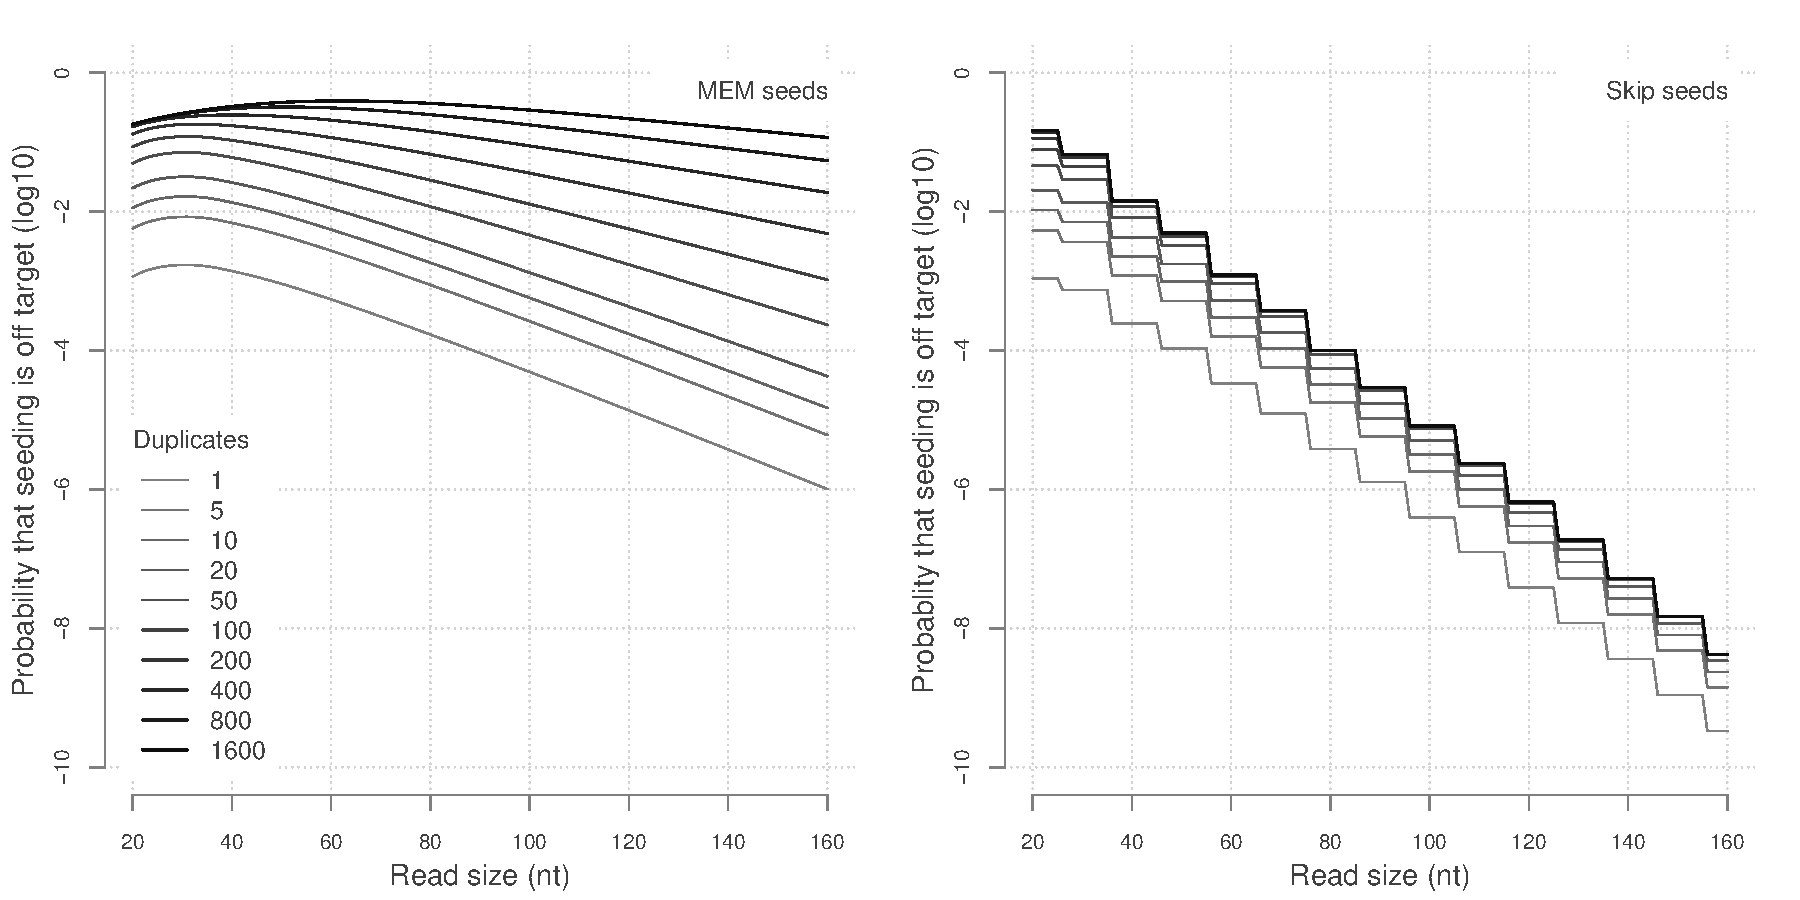
\includegraphics[scale=.41]{mortal_kombat.pdf}
\end{center}
\caption{\textbf{Comparing seeding strategies with Sesame.} Left: MEM
seeds with $\gamma=19$ and $\mu=0.06$. Right: skip-9 seeds with
$\gamma=16$ and $\mu=0.06$. The probabilities that seeding is off target
were computed using Sesame. Each curve represents the probability for a
given number of duplicates ($N$). Estimates using iterative methods (skip
seeds and MEM sees where $N \leq 20$) were computed to within 1\%
accuracy. Estimates using Monte Carlo sampling (MEM seeds where $N > 20$)
were computed as the average of 500 million simulations.
}
\label{fig_mortal_kombat}
\end{figure*}

The probabilities that seeding is off target for different read sizes $k$
and different number of duplicates $N$ are plotted in
Fig.~\ref{fig_mortal_kombat}. The left panel shows the results for MEM
seeds and the right panel shows the results for skip seeds. Here the error
rate $p$ is set to 1\%, close to the specifications the Illumina platform,
and the divergence rate between duplicates $\mu$ is set to an arbirtarry
value of 6\%.

The behaviors of the two types of seeds are dramatically different. Let us
start with MEM seeds. For every value of $N$, the probability initially
increases with the read size, and then drops exponentially. The initial
increase is a hallmark of MEM seeds; it is due to the fact that duplicates
can mask the target. Note that the asymptotic decay depends on the number
of duplicates $N$ because each duplicate can mask the target and thereby
reduces the probability that it is discovered. Overall, these results show
that the performance of MEM seeds is poor when the target has more than
approximately 20 duplicates.

Turning to skip seeds, we see that the curves have a staircase look with a
drop every 10 nucleotides. This is so because seeding probabilities remain
unchanged until there is space for another seed of size 16 on the read.
The curves are otherwise decreasing with a steady exponential trend where
the asymptotic decay does not depend on the number of duplicates $N$. The
reason is that duplicates do not prevent the target from being discovered,
they merely fool the mapper when the target was not found. This property
makes the asymptotic decay of skip seeds substantially faster that of MEM
seeds when $N$ is large.

Those properties are self evident in retrospect, but they are not
necessarily obvious from the definitions of MEM seeds and skip seeds.
Keeping in mind that the asymptotic decay depends on $N$ for MEM seeds
helps understand what their main limitation is.

Fig.~\ref{fig_mortal_kombat} suggests that skip-9 seeds of size 16 are
just better than MEM seeds of size 19. However, the gain in sensitivity
comes at the cost of a larger candidate set, slowing down the mapping
process. To remain competitive, Bowtie2 further filters the candidate set
using a priority policy. But since some candidates are not checked, the
probability that seeding is off target is larger than shown in
Figure~\ref{fig_mortal_kombat}.

\subsection{Key insights about MEM seeds}

At least two key insights about MEM seeds can be gained from
Fig.~\ref{fig_mortal_kombat}. The first is that it is probably not worth
for a MEM-based mapper to check all the candidate loci when there are more
than approximately 20 them. The mapper may find the correct location, but
even if this is the case, the mapping quality will remain low because the
prior chances of failure were high. A better strategy is to either bail
out ot not waste time or to switch to a more sensitive seeding method (BWA
opts for the second and uses a re-seeding policy). It is also important
to note that this decision should be based on an estimated value of $N$
and not, for instance, on the size of the seed or some other variable.

A second insight is that for MEM seeds, the off-target rate is always
above $10^{-3}$ for reads of 50 nucleotides or fewer. Here it is important
to mention that the value $\mu=0.06$ is not even the worst for reads of
this size when $p=0.01$ (according to Fig.~\ref{fig:curves_mem}, the worst
value is around 0.02). So if $\mu$ is unknown and one wishes to be
conservative, it seems that reads of 50 nucleotides cannot be mapped with
confidence better than $1/1000$.

However, this is not true for the reason that it is practically impossible
to map an Illumina read of size 50 to the wrong location when $N=0$ (see
section~\ref{sec:random_seeds}). This means that tweaking the seeding
method to improve the mapping quality score will have less impact than
checking whether $N$ is 0 (in other words, whether the target is a unique
sequence).

These insights suggest that there is a way to make MEM seeds more useful
for short read mappers. We are currently working on a prototype based on
these two ideas to increase the speed and the accuracy of short read
mapping. This requires estimating $N$ and $\mu$ for every read and will be
described in a separate work.


\section{Discussion}

We have devised a set of methods to compute the probability that seeding
heuristics fail and commit the mapping process to an error. We have also
implemented the solution as an open source C library to perform the
computations. This fills a knowledge gap to understand and calibrate the
performance of the seeding heuristics. The pillars of our strategy are
borrowed from analytic combinatorics~\cite{flajolet2009analytic,
sedgewick2013introduction}, even though we do not follow the complete
programme. Constructing generating functions usually serves the purpose of
finding their singularities in order to approximate the solution. In our
case, however, the weighted generating functions cannot be computed so
this strategy is not applicable.

To find the probabilities of interest in the absence of a fully specified
weighted generating function, we compute only the first terms using
iterative methods as explained in section~\ref{sec:example_skip}, or using
Monte Carlo sampling as explained in section~\ref{sec:montecarlo}. In this
regard, the breakthrough is the encoding of reads as segments in different
alphabets, which is an implicit form of Markov
imbedding~\cite{fu1994distribution}.

The methods rely on the knowledge of two essential parameters: the number
of duplicates $N$ and their divergence rate $\mu$. These quantities can be
estimated efficiently using the FM-index~\cite{ferragina2005indexing} and
we will publish the detail of this method elsewhere, together with a more
complete overview of how to use the results presented here to implement
practical mapping algorithms.

The method is general, but it is important to clearly state the
assumptions it depends on. First and most importantly, we have ignored
insertions and deletions. We assume that the sequencing errors are
substitutions only, which makes the method adapted to the Illumina
technology, but not to deletion-prone instruments such as the Oxford
Nanopore technology. We also assume that insertions and deletions never
occur among duplicated sequences. This is obviously incorrect, but our
initial tests with real data suggest that this is a minor impediment (most
likely because this is only one of several simplifying assumptions).
Incorporating insertions and deletions would make the theory intractable,
so it is presently unclear how to deal with this type of error.

The second assumption is that all the candidate locations with a seed are
tested with an exact sequence alignment algorithm, so that the best
location is always discovered if it is present in the candidate set. This
is not completely unrealistic, but it is important to note that for plant
and animal genomes, a single seed may have tens of thousands of hits.
Therefore, most mappers impose a limit on the number of alignments per
read, opening the possibility that the best hit is seeded but not aligned.
This is again a minor impediment, since we can replace the probability
that the location is false by the proportion of candidates that were not
aligned.

The third assumption is that all the duplicate sequences evolve
independently of each other and at the same rate. This is again incorrect,
because duplication events can happen continuously, creating complex
ancestry relationships. It is possible to infer the ancestry using tree
reconstruction techniques, but it would be challenging to incorporate this
information in the present theory. The symbols of the alphabets developed
above implicitly assume that the sequences are exchangeable and the
complexity of the calculations explodes if it is not the case.

The last assumption is that seeds can match only the target or one of its
duplicates. This does not hold in general but we have shown how to deal
with this possibility \textit{a posteriori} in
section~\ref{sec:random_seeds}.

Being able to compute seeding probabilities revealed some interesting
facts (sections~\ref{sec:illdual}, \ref{sec:illskipdual} and
\ref{sec:illmem}). The first is that the seeding schemes considered here
have a worst case scenario for a particular value of the divergence
between duplicates $\mu$. Importantly, the worst value varies between
different seeding methods, so it is possible in theory to construct
opportunistic seeding strategies that pick the best method for every read.

Another interesting fact is that skip seeds can have better performance
than exact seeds in the sense that they can yield lower off-seeding
probabilities. However, this always comes at the cost of accuracy because
skipping nulceotides reduces the probability of on-target seeding.

Finally, we also observed that MEM seeds cause a very serious increase in
off-target seeding compared to exact seeds and skip seeds. This does not
mean that MEM seeding is a bad strategy (it is usually faster than the
other methods), but it is a good idea to keep an eye on performance and
switch method or even skip the read altogether if the chances of
discovering the target are too low.

Regarding the methodology, the Monte Carlo approach of
algorithm~\ref{alg:mcmc} is relatively straightforward, so one may wonder
why the approach with weighted generating functions is necessary for MEM
seeds. The only reason is precision. To estimate the frequency of an event
by Monte Carlo sampling, it must occur at least a few times in the
simulation. For instance, with 1 million rounds of sampling, frequencies
around $1/100,000$ or lower cannot be measured accurately. When one is
interested only in frequent events, it is thus a reasonable strategy. On
the other hand, for $N < 20$, the probability that MEM seeding is null or
off-target is relatively small, so we need a method that is accurate in
this range. Fortunately, the transfer matrix method is fast because the
dimension of the matrix $\mathring{M}_N(z)$ is small and the computations
are not prohibitive.

The proposed methods meet the demand for speed. One needs to compute the
probabilities only once for a given value of $N$ and $\mu$ (the error rate
$p$ is known and constant). For $N > 20$, the iterative method is usually
too slow and we need to use Monte Carlo sampling instead. The running
time depends on $p$, on the size of the reads $k$, and on the desired
number of iterations. Since those are constant throughout the sequencing
run, the method always takes the same time (around 1-10 seconds for reads
of size $100$-$200$ nucleotides on modern hardware). The values of $N$ and
$\mu$ can be binned in intervals so that there are only around $100$ pairs
for a total cost of a few minutes per run. Considering that mappers can
process at most $10,000$ reads per second per core, the time of mapping a
sequencing run of 250 million reads is over 7 hours per core, two orders
of magnitude larger than the time required to estimate the probabilities
of error.

Finally, one may wonder if our approach has any advantage over methods
based on machine learning. Such algorithms have already proved
useful~\cite{lee2014mosaik} and the rapid progress in the field of deep
learning suggests that it is possible to train algorithms to accurately
estimate mapping quality. In time, such algorithms may prove faster and/or
more robust because they could learn intrinsic biases of the mapping
algorithms. Yet, the main benefit of our approach will remain: the
combinatorial constructions are a direct access to the nature of the
problem. For instance, viewing MEM seeds through the lens of hard and soft
masks turns a seemingly intractable process into a relatively simple one
(see algorithm~\ref{alg:mcmc}). The combinatorial stance is that there is
value in clarity.

In conclusion, we presented a practical solution to the problem of
estimating the probability of false positives when using seeding
heuristics. This solution is adapted for mapping short reads sequenced
with the Illumina technology. Being able to calibrate the seeding
heuristic not only allows the user to choose how to balance speed versus
accuracy, but also opens new applications. For instance, one can map reads
from contaminated samples in pools of closely related genomes
(\textit{e.g.}, modern human and Neanderthal) in order to assign the reads
to the organism they belong to. In this case, the probabilities of false
positives give the right level of confidence in the assignment.

More generally, the analytic combinatorics programme is a very powerful
tool to address problems in bioinformatics. Here we have seen how this
strategy can be useful even when the generating functions cannot be
computed. Using the same ideas, one could calibrate heuristics used in
other alignment methods, especially in the expanding field of long-read
technologies.


\section*{Acknowledgements}

We acknowledge the financial support of the Spanish Ministry of Economy,
Industry and Competitiveness (`Centro de Excelencia Severo Ochoa
2013-2017', Plan Estatal PGC2018-099807-B-I00), of the CERCA
Programme~/~Generalitat de Catalunya, and of the European Research Council
(Synergy Grant 609989). R.~C. was supported by the People Programme
(Marie Curie Actions) of the European Union's Seventh Framework Programme
(FP7/2007-2013) under REA grant agreement 608959. We also acknowledge
support of the Spanish Ministry of Economy and Competitiveness (MEIC) to
the EMBL partnership.

%---------------------------------------------------------------
%---------------------------------------------------------------

\bibliography{references,pubmed}
\bibliographystyle{unsrt}

%----------------------------------------------------------------

\end{document}

%gs -dNoOutputFonts -sDEVICE=pdfwrite -o out.pdf latex.pdf 
